%!TEX root = ../larxxia.tex


\section{Introducing linear transformations}
\label{sec:ilt}
\secttoc
\begin{comment}
\pooliv{\S3.6} \layiv{\S1.8--9} \holti{\S3.1}
\end{comment}

\index{linear transformation|(}

\begin{aside}
This optional section unifies the transformation examples seen so far, and forms a foundation for more advanced algebra. 
\end{aside}

Recall the function notation such as \(f(x)=x^2\) means that for each \(x\in\RR\), the function~\(f(x)\) gives a result in~\(\RR\), namely the value~\(x^2\), as plotted in the margin.  
\marginpar{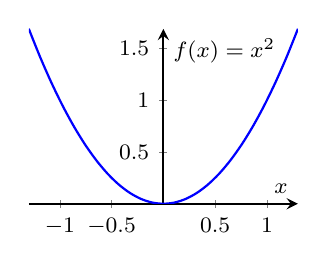
\begin{tikzpicture}
  \begin{axis}[footnotesize,font=\footnotesize
  ,xlabel={$x$}, ylabel={$f(x)=x^2$}
  ,axis lines=middle,thick,smooth,axis equal image
  ,domain=-1.3:1.3]
  \addplot+[blue,no marks]{x^2};
  \end{axis}
\end{tikzpicture}}%
We often write \(f:\RR\to\RR\) to denote this functionality: that is, \(f:\RR\to\RR\) means function~\(f\) transforms any given real number into another real number by some rule.

There is analogous functionality in multiple dimensions with vectors: given any vector 
\begin{itemize}
\item multiplication by a diagonal matrix stretches and shrinks the vector (section~\ref{sec:dmd});
\item multiplication by an orthogonal matrix rotate the vector (section~\ref{sec:omr});
and \item projection finds a vector's components in a subspace (section~\ref{sec:proj}).
\end{itemize}
Correspondingly, we use the notation \(f:\RR^n\to\RR^m\) to mean function~\(f\) transforms a given vector with \(n\)~components (in~\(\RR^n\)) into another vector with \(m\)~components (in~\(\RR^m\)) according to some rule. 
For example, suppose the function~\(f(\xv)\) is to denote multiplication by the matrix
\begin{equation*}
A=\begin{bmatrix} 1&-\frac13\\\frac12&-1\\-1&-\frac12 \end{bmatrix}.
\end{equation*}
Then the function
\begin{equation*}
f(\xv)=\begin{bmatrix} 1&-\frac13\\\frac12&-1\\-1&-\frac12 \end{bmatrix}\begin{bmatrix} x_1\\x_2 \end{bmatrix}
=\begin{bmatrix} x_1-x_2/3\\x_1/2-x_2\\-x_1-x_2/2 \end{bmatrix}.
\end{equation*}
\marginpar{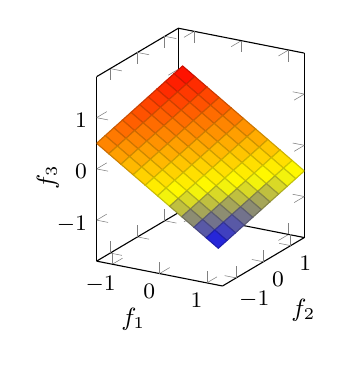
\begin{tikzpicture} 
\begin{axis}[small,font=\footnotesize
  ,axis equal image,view={30}{20}
  ,xlabel=$f_1$,ylabel=$f_2$,zlabel={$f_3$},label shift={-2ex}]
\addplot3[surf,domain=-1:1,samples=11] ({x-y/3},{x/2-y},{-x-y/2});
\end{axis}
\end{tikzpicture}}%
That is, here \(f:\RR^2\to\RR^3\).  
Given any vector in the 2D-plane, the function~\(f\), also called a \idx{transformation}, returns a vector in 3D-space.  
The marginal plot illustrates the subspace formed by this~\(f(\xv)\) for all 2D vectors~\xv.


There is a major difference between `curvaceous' functions like the parabola above, and matrix multiplication functions such as rotation and projection.
The difference is that linear algebra empowers many practical results in the latter case.



\begin{definition} \label{def:lintran} 
A \idx{transformation}\slash function \(T:\RR^n\to\RR^m\) is called a \bfidx{linear transformation} if
\begin{enumerate}
\item\label{def:lintran:i} \(T(\uv+\vv)=T(\uv)+T(\vv)\) for all \(\uv,\vv\in\RR^n\), and
\item\label{def:lintran:ii} \(T(c\vv)=cT(\vv)\) for all \(\vv\in\RR^n\) and all scalars~\(c\).
\end{enumerate}
\end{definition}


\begin{example}[1D cases] \label{eg:}
\begin{enumerate}
\item Show that the parabolic function \(f:\RR\to\RR\) where \(f(x)=x^2\) is not a linear transformation.
\begin{solution} 
To test Property~\ref{def:lintran:i}, consider \(f(x+y)=(x+y)^2=x^2+2xy+y^2=f(x)+2xy+f(y)\neq f(x)+f(y)\) for all~\(x\) and~\(y\) (it is equal if either are zero, but the test requires equality to hold for all~\(x\) and~\(y\)).  
Alternatively one could test Property~\ref{def:lintran:ii} and consider \(f(cx)=(cx)^2=c^2x^2=c^2f(x)\neq cf(x)\) for all~\(c\).
Either of these prove that \(f\)~is not a linear transformation.
\end{solution}

\item Is the function \(T(x)=|x|\), \(T:\RR\to\RR\), a linear transformation? 
\marginpar{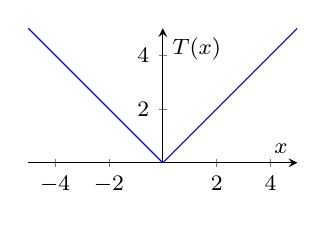
\begin{tikzpicture}
\begin{axis}[footnotesize,font=\footnotesize
,axis equal image,axis lines=middle
,xlabel={$x$},ylabel={$T(x)$}]
\addplot+[no marks]{abs(x)};
\end{axis}
\end{tikzpicture}}
\begin{solution} 
To prove not it is sufficient to find just one instance when Definition~\ref{def:lintran} fails. 
Let \(u=-1\) and \(v=2\)\,, then \(T(u+v)=|-1+2|=|1|=1\) whereas \(T(u)+T(v)=|-1|+|2|=1+2=3\neq T(u+v)\) so the function~\(T\) fails the additivity and so is not a linear transformation.
\end{solution}

\item Is the function \(g:\RR\to\RR\) such that \(g(x)=-x/2\) a linear transformation?
\marginpar{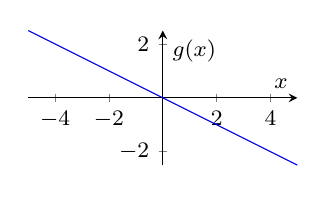
\begin{tikzpicture}
\begin{axis}[footnotesize,font=\footnotesize
,axis equal image,axis lines=middle
,xlabel={$x$},ylabel={$g(x)$}]
\addplot+[no marks]{-x/2};
\end{axis}
\end{tikzpicture}}
\begin{solution} 
Because the graph of~\(g\) is a straight line (as in the marginal picture) we suspect it is a linear transformation.
Thus check the properties in full generality:
\begin{description}
\item[\ref{def:lintran:i}] for all \(u,v\in\RR\), \(g(u+v)=-(u+v)/2=-u/2-v/2=(-u/2)+(-v/2)=g(u)+g(v)\);
\item[\ref{def:lintran:ii}] for all \(u,c\in\RR\), \(g(cu)=-(cu)/2=c(-u/2)=cg(u)\).
\end{description}
Hence \(g\) is a linear transformation.
\end{solution}

\item Show that the function \(h(y)=2y-3\), \(h:\RR\to\RR\), is not a linear transformation.
\marginpar{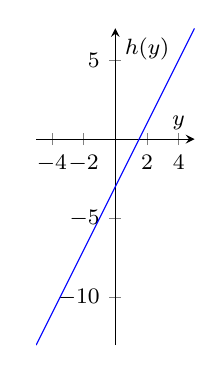
\begin{tikzpicture}
\begin{axis}[small,font=\footnotesize
,axis equal image,axis lines=middle
,xlabel={$y$},ylabel={$h(y)$}]
\addplot+[no marks]{2*x-3};
\end{axis}
\end{tikzpicture}}
\begin{solution} 
Because the graph of~\(h(y)\) is a straight line we suspect it may be a linear transformation (as shown in the margin).
To prove not it is enough to find one instance when Definition~\ref{def:lintran} fails. 
Let \(u=0\) and \(c=2\)\,, then \(h(cu)=h(2\cdot0)=h(0)=-3\) whereas \(ch(u)=2h(0)=2\cdot(-3)=-6\neq h(cu)\) so the function~\(g\) fails the multiplication rule and hence is not a linear transformation.
(This function fails because linear transformations have to pass through the origin.)
\end{solution}

\item Is the function \(S:\ZZ\to\ZZ\) given by \(S(n)=-2n\) a linear transformation?  Here \ZZ~denotes the set of integers \(\ldots,-2,-1,0,1,2,\ldots\)\,.
\marginpar{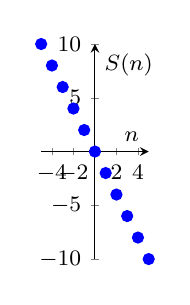
\begin{tikzpicture}
\begin{axis}[footnotesize,font=\footnotesize
,axis equal image,axis lines=middle
,xlabel={$n$},ylabel={$S(n)$}]
\addplot+[samples=11,only marks]{-2*x};
\end{axis}
\end{tikzpicture}}
\begin{solution} 
No, because the function~\(S\) is here only defined for integers~\ZZ\ (as plotted in the margin) whereas Definition~\ref{def:lintran} requires the function to be defined for all reals.
\footnote{More advanced linear algebra generalises the definition of a linear transformation to non-reals, but not here.}
\end{solution}

\end{enumerate}
\end{example}




\begin{activity}
Which of the following is the graph of a linear transformation?
\begin{parts}
\item 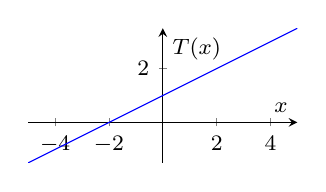
\begin{tikzpicture}
\begin{axis}[footnotesize,font=\footnotesize
,axis equal image,axis lines=middle
,xlabel={$x$},ylabel={$T(x)$}]
\addplot+[no marks]{0.5*x+1};
\end{axis}
\end{tikzpicture}

\item 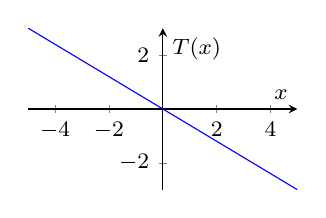
\begin{tikzpicture}
\begin{axis}[footnotesize,font=\footnotesize
,axis equal image,axis lines=middle
,xlabel={$x$},ylabel={$T(x)$}]
\addplot+[no marks]{-0.6*x};
\end{axis}
\end{tikzpicture}

\item 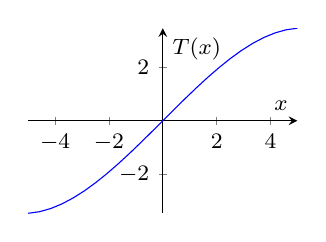
\begin{tikzpicture}
\begin{axis}[footnotesize,font=\footnotesize
,axis equal image,axis lines=middle
,xlabel={$x$},ylabel={$T(x)$}]
\addplot+[no marks]{x-x^3/80};
\end{axis}
\end{tikzpicture}

\item 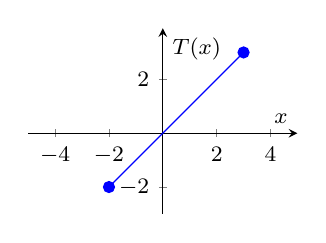
\begin{tikzpicture}
\begin{axis}[footnotesize,font=\footnotesize
,axis equal image,axis lines=middle
,xmin=-5,xmax=5,domain=-2:3,ymin=-3,ymax=3.9
,xlabel={$x$},ylabel={$T(x)$}]
\addplot+[samples=2]{x};
\end{axis}
\end{tikzpicture}

\end{parts}
\end{activity}




\begin{example}[higher-D cases] \label{eg:}
\begin{enumerate}
\item Let function \(T:\RR^3\to\RR^3\) be \(T(x,y,z)=(y,z,x)\).  
Is~\(T\) a linear transformation?
\begin{solution} 
Yes, because it satisfies the two properties:
\begin{description}
\item[\ref{def:lintran:i}] for all \(\uv=(x,y,z)\) and \(\vv=(x',y',z')\) in~\(\RR^3\) consider \(T(\uv+\vv)
=T(x+x',y+y',z+z')
=(y+y',z+z',x+x')
=(y,z,x)+(y',z',x')
=T(x,y,z)+T(x',y',z')
=T(\uv)+T(\vv)\);

\item[\ref{def:lintran:ii}] for all \(\uv=(x,y,z)\) and scalars~\(c\)
consider \(T(c\uv)
=T(cx,cy,cz)
=(cy,cz,cx)
=c(y,z,x)
=cT(x,y,z)
=cT(\uv)\).
\end{description}
Hence, \(T\) is a linear transformation.
\end{solution}

\item Consider the function \(f(x,y,z)=x+y+1\), \(f:\RR^3\to\RR\): is \(f\)~a linear transformation?
\begin{solution} 
No.  For example, choose \(\uv=\ov\) and scalar \(c=2\) then \(f(c\uv)=f(2\cdot\ov)=f(\ov)=1\) whereas \(cf(\uv)=2f(\ov)=2\cdot 1=2\)\,.
Hence~\(f\) fails the scalar multiplication property~\ref{def:lintran:ii}.
\end{solution}


\item\label{eg:LTtwoDg} Which of the following illustrated transformations of the plane \emph{cannot} be that of a linear transformation?
In each illustration of a transformation~\(T\), the four corners of the blue \idx{unit square} (\((0,0)\), \((1,0)\), \((1,1)\) and~\((0,1)\)), are transformed to the four corners of the red figure (\(T(0,0)\), \(T(1,0)\), \(T(1,1)\) and~\(T(0,1)\)---the `roof' of the unit square clarifies which side goes where).
\begin{parts}
\item\TwoDnotLT{-1.4}{1.1}{-0.5}{1.9}00
\item\TwoDnotLT{0.9}{0.3}{-0.0}{0.7}{0.2}{-0.3}
\item\TwoDnotLT{1.6}{0.4}{0.7}{1.1}{0}{0}
\item\TwoDnotLT{0.0}{1.1}{-2.0}{-0.6}{0.3}{0.1}
\item\TwoDnotLT{-1.0}{0.9}{-1.2}{0.1}{0.4}{0.2}
\item\TwoDnotLT{-0.8}{-1.4}{0.6}{-0.3}00
\end{parts}
\begin{solution} 
To \emph{test} we check the addition property~\ref{def:lintran:i}.
First, with \(\uv=\vv=\ov\) Definition~\ref{def:lintran:i} requires \(T(\ov+\ov)=T(\ov)+T(\ov)\), but the left-hand side is just~\(T(\ov)\) which cancels with one on the right-hand side to leave that a linear transformation has to satisfy \(T(\ov)=\ov\)\,: all the shown transformations satisfy \(T(\ov)=\ov\) as the (blue) origin point is transformed to the (red) origin point.
Second, with \(\uv=(1,0)\), \(\vv=(1,0)\) and \(\uv+\vv=(1,1)\) Definition~\ref{def:lintran:i} requires \(T(1,1)=T(1,0)+T(0,1)\): let's see which do not pass this test.
\begin{enumerate}
\item Here \(T(1,1)\approx(-0.3,1.4)\), whereas
\(T(1,0)+T(0,1)\approx (-1.4,-0.5)+(1.1,1.9)
=(-0.3,1.4)\approx T(1,1)\) 
so this may be a linear transformation.
\item Here \(T(1,1)\approx(1.4,0.4)\), whereas
\(T(1,0)+T(0,1)\approx (0.9,0)+(0.3,0.7)
=(1.2,0.7)\not\approx T(1,1)\) 
so this \emph{cannot} be a linear transformation.
\item Here \(T(1,1)\approx(2.0,1.8)\), whereas
\(T(1,0)+T(0,1)\approx (1.6,0.7)+(0.4,1.1)
=(2.0,1.8)\approx T(1,1)\) 
so this may be a linear transformation.
\item Here \(T(1,1)\approx(1.4,-2.5)\), whereas
\(T(1,0)+T(0,1)\approx (0,-2)+(1.1,-0.6)
=(1.1,-2.6)\not\approx T(1,1)\) 
so this \emph{cannot} be a linear transformation.
\item Here \(T(1,1)\approx(0.3,-0.9)\), whereas
\(T(1,0)+T(0,1)\approx (-1,-1.2)+(0.9,0.1)
=(-0.1,-1.1)\not\approx T(1,1)\) 
so this \emph{cannot} be a linear transformation.
\item Here \(T(1,1)\approx(-2.2,0.3)\), whereas
\(T(1,0)+T(0,1)\approx (-0.8,0.6)+(-1.4,-0.3)
=(-2.2,0.3)\approx T(1,1)\) 
so this may be a linear transformation.
\end{enumerate} 
The ones that pass this test may fail other tests: all we are sure of is that those that fail such tests \emph{cannot} be linear transformations.
\end{solution}

\item\label{eg:LTthreeDg}
The previous Example~\ref{eg:LTtwoDg} illustrated that a linear transformation of the square seems to transform the unit square to a \idx{parallelogram}: if a function transforms the unit square to something that is not a parallelogram, then the function cannot be a linear transformation.
Analogously in higher dimensions: for example, if a function transforms the unit cube to something which is not a \idx{parallelepiped}, then the function is not a linear transformation.
Using this information, which of the following illustrated functions, \(f:\RR^3\to\RR^3\), \emph{cannot} be a linear transformation?
Each of these stereo illustrations plot the \idx{unit cube} in blue (with a `roof' and `door' to help orientate), and the transform of the unit cube in red (with its transformed `roof' and `door').
% Generated these examples with x set to the unit cube coords, then
% x*(eye(3,3)+randn(3,3)*0.5)+ x.*x(:,[2 3 1])*randn(3,3)*0.4
\begin{enumerate}
\item \def\unithousesize{small}
\ThreeDgen{
   0.00   0.00   0.00 \\
   1.02   0.30   0.59 \\
   1.21   0.83   0.15 \\
   1.15   0.63   0.78 \\
   1.29   1.03   0.45 \\
   1.35   1.22  -0.17 \\
   1.49   1.61  -0.50 \\
   0.46   1.31  -1.08 \\
   0.00   0.00   0.00 \\
  -0.09  -0.32   1.04 \\
   0.93  -0.02   1.63 \\
   0.63   0.42   1.00 \\
  -0.09  -0.32   1.04 \\
   0.37   0.99  -0.04 \\
   0.63   0.42   1.00 \\
   1.40   1.29   0.54 \\
   0.37   0.99  -0.04 \\
   0.46   1.31  -1.08 \\
   1.49   1.61  -0.50 \\
   1.40   1.29   0.54 \\
   0.93  -0.02   1.63 \\
   1.02   0.30   0.59 \\
}
This \emph{may} be a linear transformation as the transform of the unit cube looks like a parallelepiped. 


\item \def\unithousesize{footnotesize}
 \ThreeDgen{
   0.00   0.00   0.00 \\
   1.60  -0.67  -0.11 \\
   1.47  -0.09  -0.12 \\
   1.19   0.35   0.22 \\
   1.09   0.83   0.22 \\
   1.38   0.34  -0.12 \\
   1.28   0.77  -0.13 \\
  -0.68   1.13  -0.14 \\
   0.00   0.00   0.00 \\
  -0.37   0.73   0.44 \\
   1.15  -0.04   0.44 \\
   0.04   1.29   0.51 \\
  -0.37   0.73   0.44 \\
  -1.09   2.14   0.32 \\
   0.04   1.29   0.51 \\
   0.79   1.68   0.44 \\
  -1.09   2.14   0.32 \\
  -0.68   1.13  -0.14 \\
   1.28   0.77  -0.13 \\
   0.79   1.68   0.44 \\
   1.15  -0.04   0.44 \\
   1.60  -0.67  -0.11 \\
  }
This \emph{cannot} be a linear transformation as the unit cube transforms to something not a parallelepiped.

\item \def\unithousesize{small}
\ThreeDgen{
   0.00   0.00   0.00 \\
   1.91   0.59  -0.79 \\
   1.55   1.05  -1.08 \\
   1.63   1.55   0.10 \\
   1.39   1.88  -0.07 \\
   1.28   1.40  -1.30 \\
   1.01   1.75  -1.52 \\
  -0.79   1.27  -0.20 \\
   0.00   0.00   0.00 \\
   0.51   0.40   2.04 \\
   1.95   1.44   1.08 \\
   0.99   1.62   1.88 \\
   0.51   0.40   2.04 \\
  -0.07   1.61   2.11 \\
   0.99   1.62   1.88 \\
   1.26   2.54   0.61 \\
  -0.07   1.61   2.11 \\
  -0.79   1.27  -0.20 \\
   1.01   1.75  -1.52 \\
   1.26   2.54   0.61 \\
   1.95   1.44   1.08 \\
   1.91   0.59  -0.79 \\
  }
This \emph{cannot} be a linear transformation as the unit cube transforms to something not a parallelepiped.

\item \def\unithousesize{footnotesize}
\ThreeDgen{
   0.00   0.00   0.00 \\
   1.33   1.22   0.60 \\
   1.20   2.11   0.53 \\
   0.81   1.91   0.87 \\
   0.71   2.57   0.81 \\
   1.10   2.78   0.47 \\
   0.99   3.45   0.42 \\
  -0.34   2.23  -0.18 \\
   0.00   0.00   0.00 \\
  -0.65  -0.34   0.57 \\
   0.69   0.88   1.17 \\
  -0.28   1.32   0.89 \\
  -0.65  -0.34   0.57 \\
  -0.99   1.89   0.39 \\
  -0.28   1.32   0.89 \\
   0.35   3.11   0.99 \\
  -0.99   1.89   0.39 \\
  -0.34   2.23  -0.18 \\
   0.99   3.45   0.42 \\
   0.35   3.11   0.99 \\
   0.69   0.88   1.17 \\
   1.33   1.22   0.60 \\
  }
This \emph{may} be a linear transformation as the transform of the unit cube looks like a parallelepiped. 
\end{enumerate}
\end{enumerate}
\end{example}




\begin{activity}
Which of the following functions \(f:\RR^3\to\RR^2\) is not a linear transformation?
\begin{enumerate}
\item \(f(x,y,z)=(0,0)\)
\item \(f(x,y,z)=(y,x+z)\)
\item \(f(x,y,z)=(2.7x+3y,1-2z)\)
\item \(f(x,y,z)=(0,13x+\pi y)\)
\end{enumerate}
\end{activity}



\begin{example} \label{eg:}
For any given nonzero vector \(\wv\in\RR^n\), prove that the projection \(P:\RR^n\to\RR^n\) by \(P(\uv)=\proj_\wv(\uv)\) is a linear transformation (as a function of~\uv).
But, for any given nonzero vector \(\uv\in\RR^n\), prove that the projection \(Q:\RR^n\to\RR^n\) by \(Q(\wv)=\proj_\wv(\uv)\) is not a linear transformation (as a function of~\wv).
\begin{solution} 
\begin{itemize}
\item Consider the two properties of Definition~\ref{def:lintran} for the function~\(P\).
\begin{description}
\item[\ref{def:lintran:i}] for all \(\uv,\vv\in\RR^n\), from Defintion~\ref{def:orthproj1} for a projection, 
\(P(\uv+\vv)
=\proj_\wv(\uv+\vv)
=\wv[\wv\cdot(\uv+\vv)]/|\wv|^2
=\wv[(\wv\cdot\uv)+(\wv\cdot\vv)]/|\wv|^2
=\wv(\wv\cdot\uv)/|\wv|^2+\wv(\wv\cdot\vv)/|\wv|^2
=\proj_\wv(\uv)+\proj_\wv(\vv)
=P(\uv)+P(\vv)\);

\item[\ref{def:lintran:ii}] for all \(\uv\in\RR^n\) and scalars~\(c\), 
\(P(c\uv)
=\proj_\wv(c\uv)
=\wv[\wv\cdot(c\uv)]/|\wv|^2
=\wv[c(\wv\cdot\uv)]/|\wv|^2
=c\big[\wv(\wv\cdot\uv)/|\wv|^2\big]
=c\proj_\wv(\uv)
=cP(\uv)\).
\end{description}
Hence, the projection~\(P\) is a linear transformation.

\item Now consider \(Q(\wv)=\proj_\wv(\uv)\).
For any \(\uv,\wv\in\RR^n\) let's check \(Q(2\wv)
=\proj_{(2\wv)}(\uv)
=(2\wv)[(2\wv)\cdot\uv]/|2\wv|^2
=4\wv(\wv\cdot\uv)/(4|\uv|^2)
=\wv(\wv\cdot\uv)/|\uv|^2
=\proj_\wv(\uv)
=Q(\wv)\neq2Q(\wv)\)
and so the projection is not a linear transformation when considered as a function of the direction of the transform~\wv\ for some given~\uv.
\end{itemize}
\end{solution}
\end{example}







\subsection{Matrices correspond to linear transformations}

One important class of linear transformations are the transformations that can be written as matrix multiplications.
The reason for the importance is that Theorem~\ref{thm:matlintran} establishes all linear transformations may be written as matrix multiplications!
This in turn justifies why we define matrix multiplication to be as it is (section~\ref{sec:amwm}): \emph{matrix multiplication is defined just so that all linear transformations are encompassed}.

\begin{example} \label{eg:}
But first, the following Theorem~\ref{thm:mattranlin} proves, among many other possibilities, that the following are linear transformations:
\begin{itemize}
\item stretching\slash shrinking along coordinate axes as these are multiplication by a diagonal matrix (section~\ref{sec:dmd});
\item rotations and/or reflections as they arise as multiplications by an orthogonal matrix (section~\ref{sec:omr});
\item orthogonal projection onto a subspace as all such projections may be expressed as multiplication by a matrix (the matrix~\(W\tr W\) in Theorem~\ref{thm:projmat}).
\end{itemize}
\end{example}


\begin{theorem} \label{thm:mattranlin} 
Let \(A\) be a given \(m\times n\) matrix and define the transformation \(T_A:\RR^n\to\RR^m\)  by the matrix multiplication \(T_A(\xv):=A\xv\) for all \(\xv\in\RR^n\). 
Then \(T_A\)~is a \idx{linear transformation}.
\end{theorem}
\begin{proof} 
Let vectors \(\uv,\vv\in\RR^n\) and scalar \(c\in\RR\) and consider the two properties of Definition~\ref{def:lintran}.
\begin{itemize}
\item[\ref{def:lintran:i}.] By the distributivity of matrix-vector multiplication (Theorem~\ref{thm:pasm}), \(T_A(\uv+\vv)=A(\uv+\vv)=A\uv+A\vv=T_A(\uv)+T_A(\vv)\).
\item[\ref{def:lintran:ii}.] By commutativity of scalar multiplication (Theorem~\ref{thm:pmm}), \(T_A(c\uv)=A(c\uv)=c(A\uv)=cT_A(\uv)\).
\end{itemize}
Hence \(T_A\)~is a linear transformation.
\end{proof}



\begin{example} \label{eg:}
Prove that a matrix multiplication with a nonzero shift~\bv, \(S:\RR^n\to\RR^m\) where \(S(\xv)=A\xv+\bv\) for vector \(\bv\neq\ov\), is not a linear transformation.
\begin{solution} 
Just consider the addition property~\ref{def:lintran:i} for the zero vectors \(\uv=\vv=\ov\):  
on the one hand, \(S(\uv+\vv)=S(\ov+\ov)=S(\ov)=A\ov+\bv=\bv\); 
on the other hand \(S(\uv)+S(\vv)=S(\ov)+S(\ov)=A\ov+\bv+A\ov+\bv=2\bv\).  
Hence when the shift~\bv\ is nonzero, there are vectors for which \(S(\uv+\vv)\neq S(\uv)+S(\vv)\) and so \(S\)~is not a linear transformation.
\end{solution}
\end{example}



Now let's establish the important converse to Theorem~\ref{thm:mattranlin}: every linear transformation can be written as a matrix multiplication.

\begin{theorem} \label{thm:matlintran} 
Let \(T:\RR^n\to\RR^m\) be a \idx{linear transformation}.
Then \(T\)~is the transformation corresponding to the \(m\times n\)  matrix
\begin{equation*}
A=\begin{bmatrix} T(\ev_1)& T(\ev_2)&\cdots&T(\ev_n) \end{bmatrix}
\end{equation*}
where \(\ev_j\) are the \idx{standard unit vector}s in~\(\RR^n\).
This matrix~\(A\), often denoted~\([T]\), is called the \bfidx{standard matrix} of the \idx{linear transformation}~\(T\).
\end{theorem}
\begin{proof} 
Let \xv\ be any vector in~\(\RR^n\): then \(\xv=(\hlist xn)=\lincomb x\ev n\) for standard unit vectors \hlist\ev n\,.
Then
\begin{eqnarray*}
T(\xv)&=&T(\lincomb x\ev n)
\\&&(\text{using the identity of Exercise~\ref{ex:genlintran}})
\\&=&x_1T(\ev_1)+x_2T(\ev_2)+\cdots+x_nT(\ev_n)
\\&=&\begin{bmatrix} T(\ev_1)& T(\ev_2)&\cdots&T(\ev_n) \end{bmatrix}
\begin{bmatrix} x_1\\x_2\\\vdots\\x_n \end{bmatrix}
\\&=&A\xv
\end{eqnarray*}
for matrix~\(A\) of the theorem.
Since \(T(\ev_1), T(\ev_2),\ldots,T(\ev_n)\) are \(n\) (column) vectors in~\(\RR^m\), the matrix~\(A\) is \(m\times n\).
\end{proof}


\begin{example} \label{eg:stmatlt}
\begin{enumerate}
\item Find the standard matrix of the linear transformation \(T:\RR^3\to\RR^4\) where \(T(x,y,z)=(y,z,x,3x-2y+z)\).
\begin{solution} 
We need to find the transform of the three standard unit vectors in~\(\RR^3\):
\begin{eqnarray*}
&&T(\ev_1)=T(1,0,0)=(0,0,1,3);
\\&&T(\ev_2)=T(0,1,0)=(1,0,0,-2);
\\&&T(\ev_3)=T(0,0,1)=(0,1,0,1).
\end{eqnarray*}
Form the standard matrix with these as its three columns, in order,
\begin{equation*}
[T]=\begin{bmatrix} T(\ev_1)&T(\ev_2)&T(\ev_3) \end{bmatrix}
=\begin{bmatrix} 0&1&0\\0&0&1\\1&0&0\\ 3&-2&1\end{bmatrix}.
\end{equation*}
\end{solution}

\item\label{eg:stmatlt:b} Find the standard matrix of the rotation of the plane by~\(60^\circ\) about the origin.
\begin{solution} 
Denote the rotation of the plane by the function \(R:\RR^2\to\RR^2\).
Since \(60^\circ=\frac\pi3\) then, as illustrated in the margin,
\marginpar{\TwoD{0.5}{-0.866}{0.866}{0.5}}%
\begin{eqnarray*}
&&R(\ev_1)=(\cos\tfrac\pi3,\sin\tfrac\pi3)
=(\tfrac12,\tfrac{\sqrt3}2),
\\&&R(\ev_2)=(-\sin\tfrac\pi3,\cos\tfrac\pi3)
=(-\tfrac{\sqrt3}2,\tfrac12).
\end{eqnarray*}
Form the standard matrix with these as its columns, in order,
\begin{equation*}
[R]=\begin{bmatrix} R(\ev_1)&R(\ev_2) \end{bmatrix}
=\begin{bmatrix} \frac12&-\frac{\sqrt3}2
\\\frac{\sqrt3}2&\frac12 \end{bmatrix}.
\end{equation*}
\end{solution}

\item Find the standard matrix of the rotation about the point~\((1,0)\) of the plane by~\(45^\circ\).
\begin{solution} 
Since the origin~\((0,0)\) is transformed by the rotation to~\((1,-1)\) which is nonzero, this transformation cannot be of the form~\(A\xv\), so cannot have a standard matrix, and hence is not a linear transformation.
\end{solution}


\item Estimate the standard matrix for each of the illustrated transformations given they transform the unit square as shown.
\def\unithousesize{footnotesize,grid}
\newcommand{\TwoDmat}[4]{\TwoD{#1}{#2}{#3}{#4}
\\\emph{Solution:} Here \(T(1,0)\approx(#1,#3)\) and \(T(0,1)\approx(#2,#4)\) so the approximate standard matrix is \(\begin{bmatrix} #1&#2\\#3&#4 \end{bmatrix}\).}
\begin{parts}
\item\TwoDmat{-2.2}{-4.8}{0.8}{-3.6}
\item\TwoDmat{0.6}{1.3}{0.3}{1.4}
\item\TwoDmat{0.2}{-1.8}{-0.7}{0.8}
\item\TwoDmat{-1.4}{0.5}{0.2}{1.7}
\item\TwoDmat{-0.1}{-0.7}{0.6}{0.2}
\item\TwoDmat{0}{-2.1}{1.0}{-0.7}
\end{parts}

\end{enumerate}
\end{example}




\begin{activity}
Which of the following is the standard matrix for the transformation \(T(x,y,z)=(4.5y-1.6z,1.9x-2z)\)?
\begin{parts}
\item \(\begin{bmatrix} 4.5&-1.6\\1.9&-2 \end{bmatrix}\)
\item \(\begin{bmatrix} 4.5&1.9\\-1.6&-2 \end{bmatrix}\)
\item \(\begin{bmatrix} 0&1.9\\4.5&0\\-1.6&-2 \end{bmatrix}\)
\item \(\begin{bmatrix} 0&4.5&-1.6\\1.9&0&-2 \end{bmatrix}\)
\end{parts}
\end{activity}




\begin{example} \label{eg:stretchLT}
For a fixed scalar~\(a\), let the function \(H:\RR^n\to\RR^n\) be \(H(\uv)=a\uv\)\,.  Show that~\(H\) is a linear transformation, and then find its standard matrix.
\begin{solution} 
Let \(\uv,\vv\in\RR^n\) and \(c\)~be any scalar.
Function~\(H\) is a linear transformation because
\begin{itemize}
\item \(H(\uv+\vv)=a(\uv+\vv)=a\uv+a\vv=H(\uv)+H(\vv)\), and
\item \(H(c\uv)=a(c\uv)=(ac)\uv=(ca)\uv=c(a\uv)=cH(\uv)\).
\end{itemize}
To find the standard matrix consider
\begin{eqnarray*}
&&H(\ev_1)=a\ev_1=(a,0,0,\ldots,0),
\\&&H(\ev_2)=a\ev_2=(0,a,0,\ldots,0),
\\&&\qquad\vdots
\\&&H(\ev_n)=a\ev_n=(0,0,\ldots,0,a).
\end{eqnarray*}
Hence the standard matrix \([H]=\diag(a,a,\ldots,a)=aI_n\).
\begin{eqnarray*}
[H]&=&\begin{bmatrix} H(\ev_1)&H(\ev_2)&\cdots&H(\ev_n) \end{bmatrix}
\\&=&\begin{bmatrix} a&0&\cdots&0
\\0&a&&0
\\\vdots&&\ddots&\vdots
\\0&0&\cdots&a \end{bmatrix}
=aI_n\,.
\end{eqnarray*}

\end{solution}
\end{example}

Consider this last Example~\ref{eg:stretchLT} in the case \(a=1\)\,: then \(H(\uv)=\uv\) is the identity and so the example shows that the standard matrix of the identity transformation is~\(I_n\).



\begin{comment} 
Could introduce kernel, range, etc as a reminder of nullspace, \idx{range}, \idx{dimension}, rank theorem.  
Omit here as the extra terminology may be confusing.  
Best to introduce such terms in subsequent abstract vector spaces and a detailed LT section.
\end{comment}
%
%\begin{definition} \label{def:} 
%Let \(T:\RR^n\to\RR^m\) be a \idx{linear transformation}.
%\begin{enumerate}
%\item The \bfidx{kernel} of~\(T\), denoted \(\ker T\), is the set of all vectors \(\uv\in\RR^n\) such that \(T(\uv)=\ov\)\,.
%\item Define the \bfidx{nullity} of~\(T\) to be the \idx{dimension} of the kernel of~\(T\).
%\item The \bfidx{range} of~\(T\), denoted \(\range T\), is the set of all vectors \(\vv\in\RR^m\) such that \(\vv=T(\uv)\) for some \(\uv\in\RR^n\).
%\item Define the \bfidx{rank} of~\(T\) to be the \idx{dimension} of the range of~\(T\).
%\end{enumerate}
%\end{definition}
%
%\begin{remark} 
%Recall the corresponding properties for matrices.
%\end{remark}
%
%
%\begin{theorem} \label{thm:} 
%Let \(T:\RR^n\to\RR^m\) be a \idx{linear transformation} with \idx{standard matrix}~\(A=[T]\) (\(m\times n\)).
%\begin{enumerate}
%\item \(\ker T\) is the \idx{nullspace} of~\(A\).
%\item \(\range T\) is the column space~\(A\).
%\item \(\rank T=\rank A\)\,.
%\item  \(\nullity T=\nullity A\)\,.
%\item The \idx{dimension} theorem: \(\rank T+\nullity T=n\)\,.
%\end{enumerate}
%\end{theorem}
%\begin{proof} Could be abstract \pooliv{p.484--6}.  Or better is direct from the standard matrix.
%\end{proof}




\subsection{The pseudo-inverse of a matrix}

\index{pseudo-inverse|(}

In solving inconsistent linear equations, \(A\xv=\bv\) for some given~\(A\)\,, Procedure~\ref{pro:appsol} finds a solution~\xv\ that depends upon the right-hand side~\bv.
\begin{aside}
This subsection is an optional extension.
\end{aside}
That is, any given~\bv\ is transformed by the procedure to some result~\xv: the result is a function of the given~\bv.
This section establishes the resulting solution given by the procedure is a linear transformation of~\bv, and hence there must be a matrix, say~\(A^+\), corresponding to the procedure. 
This matrix gives the resulting solution \(\xv=A^+\bv\)\,.
We call the matrix~\(A^+\) the \idx{pseudo-inverse} of~\(A\).

\begin{example} \label{eg:psinv34}
Find the \idx{pseudo-inverse} of the matrix \(A=\begin{bmatrix} 3\\4 \end{bmatrix}\).
\begin{solution} 
Apply Procedure~\ref{pro:appsol} to solve \(Ax=\bv\) for any right-hand side~\bv.
\begin{enumerate}
\item This matrix has an \svd\ 
\begin{equation*}
A=\begin{bmatrix} 3\\4 \end{bmatrix}
=\begin{bmatrix} \frac35&-\frac45\\\frac45&\frac35 \end{bmatrix}
\begin{bmatrix} 5\\0 \end{bmatrix}\tr{\begin{bmatrix} 1 \end{bmatrix}}
=\usv.
\end{equation*}

\item Hence \(\zv=\tr U\bv=\begin{bmatrix} \tfrac35b_1+\tfrac45b_2\\-\tfrac45b_1+\tfrac35b_2 \end{bmatrix}\).
\item Then the diagonal system \(Sy=\zv\) is \(\begin{bmatrix} 5\\0 \end{bmatrix}y=\begin{bmatrix} \tfrac35b_1+\tfrac45b_2\\-\tfrac45b_1+\tfrac35b_2 \end{bmatrix}\): approximately solve by neglecting the second component in the equations, and so from the first component just set \(y=\tfrac3{25}b_1+\tfrac4{25}b_2\)\,.
\item Then the procedure's solution is \(x=Vy=1(\tfrac3{25}b_1+\tfrac4{25}b_2)=\tfrac3{25}b_1+\tfrac4{25}b_2\)\,.
\end{enumerate}
That is, for all right-hand side vectors~\bv, this \idx{least square} solution
\begin{equation*}
x=A^+\bv\quad\text{for pseudo-inverse }A^+=\begin{bmatrix} \tfrac3{25}& \tfrac4{25} \end{bmatrix}.
\end{equation*}
\end{solution}
\end{example}



\begin{activity}
By finding the smallest magnitude, least-square, solution to \(D\xv=\bv\) for matrix \(D=\begin{bmatrix} 5&0\\0&0 \end{bmatrix}\) and arbitrary~\bv, determine that the pseudo-inverse of the diagonal matrix~\(D\) is which of the following?
\begin{parts}
\item \(\begin{bmatrix} 0.2&0\\0&0 \end{bmatrix}\)%%%%%%
\item \(\begin{bmatrix} 0&0.2\\0&0 \end{bmatrix}\)
\item \(\begin{bmatrix} 0&0\\0.2&0 \end{bmatrix}\)
\item \(\begin{bmatrix} 0&0\\0&0.2 \end{bmatrix}\)
\end{parts}
\end{activity}




A pseudo-inverse~\(A^+\) of a non-invertible matrix~\(A\) is only an `inverse' because the pseudo-inverse builds in extra information that we \emph{sometimes choose} to be desirable.
This extra information rationalises all the contradictions encountered in trying to construct an inverse of a non-invertible matrix.  
Namely, for some applications we \emph{choose} to desire that the pseudo-inverse solves the \emph{nearest} consistent system to the one specified, and we  \emph{choose} the smallest of all possibilities then allowed.
However, although there are many situations where these choices are useful, beware that there are also many situations where such choices are not appropriate.
That is, although sometimes the pseudo-inverse is useful, beware that often the pseudo-inverse is not appropriate.


\begin{theorem}[pseudo-inverse] \label{thm:lsqlt}
For a given \(m\times n\) matrix~\(A\) and in the context of wanting to solve \(A\xv=\bv\)\,, Procedure~\ref{pro:appsol} forms a \idx{linear transformation} \(T:\RR^m\to\RR^n\) to find the smallest solution~\xv\ (Theorem~\ref{thm:smallsoln}) to the closest consistent system \(A\xv=\tilde\bv\) (Theorem~\ref{thm:appsol}).
This linear transformation has an \(n\times m\) \idx{standard matrix}~\(A^+\) called the \bfidx{pseudo-inverse}, or \bfidx{Moore--Penrose inverse}, of matrix~\(A\).
\end{theorem}

\begin{proof} 
First, for each right-hand side vector~\bv\ in~\(\RR^m\), the procedure gives a result~\xv\ in~\(\RR^n\) and so is some function \(T:\RR^m\to\RR^n\).
We proceed to confirm that Procedure~\ref{pro:appsol} satisfies the two defining properties of a linear transformation (Definition~\ref{def:lintran}).
For each of any two right-hand side vectors \(\bv',\bv''\in\RR^m\) let Procedure~\ref{pro:appsol} generate similarly dashed intermediaries (\(\zv',\zv'',\yv',\yv''\)) through to two corresponding least square solutions~\(\xv',\xv''\in\RR^n\).
That is, \(\xv'=T(\bv')\) and \(\xv''=T(\bv'')\).
Throughout let the matrix~\(A\) have \svd\ \(A=\usv\) and set \(r=\rank A\)\,.
\begin{description}
\item[\ref{def:lintran:i}]  
To check \(T(\bv'+\bv'')=T(\bv')+T(\bv'')\), apply the procedure when the right-hand side is \(\bv=\bv'+\bv''\):
\begin{enumerate}\stepcounter{enumi}
\item solve \(U\zv=\bv\) by \(\zv=\tr U\bv=\tr U(\bv'+\bv'')=\tr U\bv'+\tr U\bv''=\zv'+\zv''\);
\item \begin{itemize}
\item for \(i=1,\ldots,r\) set \(y_i=z_i/\sigma_i=(z'_i+z''_i)/\sigma_i=z'_i/\sigma_i+z''_i/\sigma_i=y'_i+y''_i\), and
\item for \(i=r+1,\ldots,n\) set the free variables \(y_i=0=0+0=y'_i+y''_i\) to obtain the smallest solution (Theorem~\ref{thm:smallsoln}),;
\end{itemize}
and hence \(\yv=\yv'+\yv''\);
\item solve \(\xv=\tr V\yv\) with \(\xv=V\yv=V(\yv'+\yv'')=V\yv'+V\yv''=\xv'+\xv''\).
\end{enumerate}
Since result \(\xv=\xv'+\xv''\), thus \(T(\bv'+\bv'')=T(\bv')+T(\bv'')\).

\item[\ref{def:lintran:ii}]  
To check \(T(c\bv')=cT(\bv')\) for any scalar~\(c\), apply the procedure when the right-hand side is \(\bv=c\bv'\):
\begin{enumerate}\stepcounter{enumi}
\item solve \(U\zv=\bv\) by \(\zv=\tr U\bv=\tr U(c\bv')=c\tr U\bv'=c\zv'\);
\item \begin{itemize}
\item for \(i=1,\ldots,r\) set \(y_i=z_i/\sigma_i=(cz'_i)/\sigma_i=c(z'_i/\sigma_i)=cy'_i\), and
\item for \(i=r+1,\ldots,n\) set the free variables \(y_i=0=c0=cy'_i\) to obtain the smallest solution (Theorem~\ref{thm:smallsoln}),
\end{itemize}
and hence \(\yv=c\yv'\);
\item solve \(\xv=\tr V\yv\) with \(\xv=V\yv=V(c\yv')=cV\yv'=c\xv'\).
\end{enumerate}
Since the result \(\xv=c\xv'\), consequently \(T(c\bv')=cT(\bv')\).
\end{description}
Since Procedure~\ref{pro:appsol}, denoted by~\(T\), is a linear transformation \(T:\RR^m\to\RR^n\), Theorem~\ref{thm:matlintran} assures us \(T\)~has a corresponding \(n\times m\) standard matrix which we denote~\(A^+\) and call the \idx{pseudo-inverse}.
\end{proof}




\begin{example} \label{eg:}
Find the \idx{pseudo-inverse} of the matrix \(A=\begin{bmatrix} 5&12 \end{bmatrix}\).
\begin{solution} 
Apply Procedure~\ref{pro:appsol} to solve \(A\xv=b\) for any right-hand side~\(b\).
\begin{enumerate}
\item This matrix has an \svd\ 
\begin{equation*}
A=\begin{bmatrix} 5&12 \end{bmatrix}
=\begin{bmatrix} 1 \end{bmatrix}
\begin{bmatrix} 13& 0 \end{bmatrix}
\tr{\begin{bmatrix} \frac5{13}&-\frac{12}{13}\\\frac{12}{13}&\frac5{13} \end{bmatrix}}
=\usv.
\end{equation*}

\item Hence \(z=\tr Ub=1b=b\).
\item The diagonal system \(S\yv=z\) becomes \(\begin{bmatrix} 13&0 \end{bmatrix}\yv=b\) with general solution \(\yv=(b/13,y_2)\).
The smallest of these solutions is \(\yv=(b/13,0)\).
\item Then the procedure's result is 
\begin{equation*}
\xv=V\yv=\begin{bmatrix} \frac5{13}&-\frac{12}{13}\\\frac{12}{13}&\frac5{13} \end{bmatrix}\begin{bmatrix} b/13\\0 \end{bmatrix}
=\begin{bmatrix} \frac5{169}b\\-\frac{12}{169}b \end{bmatrix}.
\end{equation*}

\end{enumerate}
That is, for all right-hand sides~\(b\), this procedure's result is
\begin{equation*}
\xv=A^+b\quad\text{for pseudo-inverse }A^+=\begin{bmatrix} \frac5{169}\\-\frac{12}{169} \end{bmatrix}.
\end{equation*}
\end{solution}
\end{example}




\begin{activity}
Following the steps of Procedure~\ref{pro:appsol}, Find the pseudo-inverse of the matrix {\small\(\begin{bmatrix} 1&1\\2&2 \end{bmatrix}\)} given that the matrix has the \svd
\begin{equation*}
\begin{bmatrix} 1&1\\2&2 \end{bmatrix}
=\begin{bmatrix} \frac1{\sqrt5}&-\frac2{\sqrt5}
\\\frac2{\sqrt5}&\frac1{\sqrt5} \end{bmatrix}
\begin{bmatrix} 10&0\\0&0 \end{bmatrix}
\tr{\begin{bmatrix} \frac1{\sqrt2}&-\frac1{\sqrt2}
\\\frac1{\sqrt2}&\frac1{\sqrt2} \end{bmatrix}}
\end{equation*}
The pseudo-inverse is which of these?
\begin{parts}
\item \(\begin{bmatrix} 0.1&0.1\\0.2&0.2 \end{bmatrix}\)
\item \(\begin{bmatrix} 0.1&-0.1\\-0.2&0.2 \end{bmatrix}\)
\item \(\begin{bmatrix} 0.1&0.2\\0.1&0.2 \end{bmatrix}\)%%%%%%
\item \(\begin{bmatrix} 0.1&-0.2\\-0.1&0.2 \end{bmatrix}\)
\end{parts}
\end{activity}





\begin{example} \label{ex:} 
Recall that Example~\ref{eg:fourwts} explored how to best determine a  weight from four apparently contradictory measurements.
The exploration showed that Procedure~\ref{pro:appsol} agrees with the traditional method of simple averaging.
Let's see that the pseudo-inverse implements the simple average of the four measurements.

Recall that Example~\ref{eg:fourwts} sought to solve an inconsistent system \(Ax=\bv\)\,, specifically
\begin{equation*}
\begin{bmatrix} 1\\1\\1\\1 \end{bmatrix}x
=\begin{bmatrix} 84.8\\84.1\\84.7\\84.4 \end{bmatrix}.
\end{equation*}
To find the pseudo-inverse of the left-hand side matrix~\(A\), seek to solve the system for arbitrary right-hand side~\bv.
\begin{enumerate}
\item As used previously, this matrix~\(A\) of ones has an \svd\ of
\def\h{\frac12}
\begin{equation*}
A=\begin{bmatrix} 1\\1\\1\\1 \end{bmatrix}
=\begin{bmatrix} \h&\h&\h&\h
\\\h&\h&-\h&-\h
\\\h&-\h&-\h&\h
\\\h&-\h&\h&-\h \end{bmatrix}
\begin{bmatrix} 2\\0\\0\\0 \end{bmatrix}
\tr{\begin{bmatrix} 1 \end{bmatrix}}
=\usv.
\end{equation*}

\item Solve \(U\zv=\bv\) by computing 
\begin{eqnarray*}
\zv&=&\tr U\bv
=\begin{bmatrix} 
  \h&\h&\h&\h
\\\h&\h&-\h&-\h
\\\h&-\h&-\h&\h
\\\h&-\h&\h&-\h \end{bmatrix}\bv
\\&=&\begin{bmatrix} \h b_1+\h b_2+\h b_3+\h b_4
\\\h b_1+\h b_2-\h b_3-\h b_4
\\\h b_1-\h b_2-\h b_3+\h b_4
\\\h b_1-\h b_2+\h b_3-\h b_4 \end{bmatrix}.
\end{eqnarray*}

\item  Now try to solve \(Sy=\zv\)\,, that is,
\begin{equation*}
\begin{bmatrix} 2\\0\\0\\0 \end{bmatrix}y
=\begin{bmatrix} \h b_1+\h b_2+\h b_3+\h b_4
\\\h b_1+\h b_2-\h b_3-\h b_4
\\\h b_1-\h b_2-\h b_3+\h b_4
\\\h b_1-\h b_2+\h b_3-\h b_4 \end{bmatrix}.
\end{equation*}
Instead of seeking an \emph{exact} solution,  we \emph{have to} adjust the last three components to zero. 
Hence we find a solution to a slightly different problem by solving
\begin{equation*}
\begin{bmatrix} 2\\0\\0\\0 \end{bmatrix}y
=\begin{bmatrix} \h b_1+\h b_2+\h b_3+\h b_4\\0\\0\\0 \end{bmatrix},
\end{equation*}
\def\h{\frac14}%
with solution \(y=\h b_1+\h b_2+\h b_3+\h b_4\)\,.

\item Lastly, solve \(\tr Vx=y\) by computing 
\begin{equation*}
x=Vy=1y=\h b_1+\h b_2+\h b_3+\h b_4
=\begin{bmatrix} \h&\h&\h&\h \end{bmatrix}\bv\,.
\end{equation*}
\end{enumerate}
\def\h{\frac14}%
Hence the pseudo-inverse of matrix~\(A\) is \(A^+=\begin{bmatrix}  \h&\h&\h&\h\end{bmatrix}\).
Multiplication by this pseudo-inverse implements the traditional answer of averaging measurements.
\end{example}






\begin{example} \label{ex:} 
Recall that Example~\ref{eg:rstp3} rates three table tennis players, Anne, Bob and Chris.  
The rating involved solving the inconsistent system \(A\xv=\bv\) for the particular matrix and vector
\begin{equation*}
\begin{bmatrix} 1&-1&0\\1&0&-1\\0&1&-1 \end{bmatrix}\xv
=\begin{bmatrix} 1\\2\\2 \end{bmatrix}.
\end{equation*}
Find the pseudo-inverse of this matrix~\(A\).
Use the pseudo-inverse to rate the players in the cases of Examples~\ref{eg:rstp} and~\ref{eg:rstp3}.
\begin{solution} 
To find the pseudo-inverse, follow Procedure~\ref{pro:appsol} with a general right-hand side vector~\bv.
\begin{enumerate}
\item Compute an \svd\ \(A=\usv\) in \script\ with \verb|[U,S,V]=svd(A)|:
\begin{verbatim}
U =
    0.4082   -0.7071    0.5774
   -0.4082   -0.7071   -0.5774
   -0.8165   -0.0000    0.5774
S =
    1.7321         0         0
         0    1.7321         0
         0         0    0.0000
V =
    0.0000   -0.8165    0.5774
   -0.7071    0.4082    0.5774
    0.7071    0.4082    0.5774
\end{verbatim}
Upon recognising various square-roots, these matrices are
\begin{eqnarray*}
U&=&\begin{bmatrix} \frac1{\sqrt6}&-\frac1{\sqrt2}&\frac1{\sqrt3}
\\-\frac1{\sqrt6}&-\frac1{\sqrt2}&-\frac1{\sqrt3}
\\-\frac2{\sqrt6}&0&\frac1{\sqrt3} \end{bmatrix},
\\
S&=&\begin{bmatrix} \sqrt3&0&0
\\0&\sqrt3&0
\\0&0&0 \end{bmatrix},
\\
V&=&\begin{bmatrix} 0&-\frac2{\sqrt6}&\frac1{\sqrt3}
\\-\frac1{\sqrt2}&\frac1{\sqrt6}&\frac1{\sqrt3}
\\\frac1{\sqrt2}&\frac1{\sqrt6}&\frac1{\sqrt3} \end{bmatrix}.
\end{eqnarray*}
The system of equations for the ratings becomes
\begin{equation*}
A\xv=
U\underbrace{S\overbrace{\tr V\xv}^{=\yv}}_{=\zv}
=\bv.
\end{equation*}

\item As \(U\) is orthogonal, \(U\zv=\bv\) has unique solution 
\begin{equation*}
\zv=\tr U\bv=\begin{bmatrix} \frac1{\sqrt6}&-\frac1{\sqrt6}&-\frac2{\sqrt6}
\\-\frac1{\sqrt2}&-\frac1{\sqrt2}&0
\\\frac1{\sqrt3}&-\frac1{\sqrt3}&\frac1{\sqrt3} \end{bmatrix}\bv
\,.
\end{equation*}


\item Now solve \(S\yv=\zv\).
But \(S\) has a troublesome zero on the diagonal. 
So interpret the equation \(S\yv=\zv\) in detail as
\begin{equation*}
\begin{bmatrix} \sqrt3&0&0
\\0&\sqrt3&0
\\0&0&0 \end{bmatrix}\yv=\begin{bmatrix} \frac1{\sqrt6}&-\frac1{\sqrt6}&-\frac2{\sqrt6}
\\-\frac1{\sqrt2}&-\frac1{\sqrt2}&0
\\\frac1{\sqrt3}&-\frac1{\sqrt3}&\frac1{\sqrt3} \end{bmatrix}\bv:
\end{equation*}
\begin{enumerate}
\item the first line requires \(y_1=\frac1{\sqrt3}\begin{bmatrix} \frac1{\sqrt6}&-\frac1{\sqrt6}&-\frac2{\sqrt6} \end{bmatrix}\bv
=\frac13\begin{bmatrix} \frac1{\sqrt2}&-\frac1{\sqrt2}&-\sqrt2 \end{bmatrix}\);
\item the second line requires \(y_2=\frac1{\sqrt3}\begin{bmatrix} -\frac1{\sqrt2}&-\frac1{\sqrt2}&0\end{bmatrix}\bv
=\begin{bmatrix} -\frac1{\sqrt6}&-\frac1{\sqrt6}&0\end{bmatrix}\bv\);
\item the third line requires \(0y_3=\begin{bmatrix} \frac1{\sqrt3}&-\frac1{\sqrt3}&\frac1{\sqrt3} \end{bmatrix}\bv\) which generally cannot be satisfied, so we set \(y_3=0\) to get the \emph{smallest solution of the system after projecting~\bv\ onto the column space of~\(A\)}.
\end{enumerate}

\item Finally, as \(V\) is orthogonal, \(\tr V\xv=\yv\) has the solution \(\xv=V\yv\) (unique for each valid~\yv):
\begin{eqnarray*}
\xv&=&V\yv
\\&=&\begin{bmatrix} 0&-\frac2{\sqrt6}&\frac1{\sqrt3}
\\-\frac1{\sqrt2}&\frac1{\sqrt6}&\frac1{\sqrt3}
\\\frac1{\sqrt2}&\frac1{\sqrt6}&\frac1{\sqrt3} \end{bmatrix}
\begin{bmatrix} \frac1{3\sqrt2}&-\frac1{3\sqrt2}&-\frac{\sqrt2}3 
\\-\frac1{\sqrt6}&-\frac1{\sqrt6}&0
\\0&0&0 \end{bmatrix}\bv
\\&=&\frac13\begin{bmatrix} 1&1&0
\\-1&0&1
\\0& -1&-1 \end{bmatrix}\bv
\end{eqnarray*}
\end{enumerate}
Hence the pseudo-inverse of~\(A\) is
\begin{equation*}
A^+=\frac13\begin{bmatrix} 1&1&0
\\-1&0&1
\\0& -1&-1 \end{bmatrix}.
\end{equation*}
\begin{itemize}
\item In Example~\ref{eg:rstp}, Anne beat Bob
3-2 games; Anne beat Chris 3-1; Bob beat Chris 3-2 so the right-hand side vector is \(\bv=(1,2,1)\).
The procedure's ratings are then, as before, 
\begin{equation*}
\xv=A^+\bv=\frac13\begin{bmatrix} 1&1&0
\\-1&0&1
\\0& -1&-1 \end{bmatrix}\begin{bmatrix} 1\\2\\1 \end{bmatrix}
=\begin{bmatrix} 1\\0\\-1 \end{bmatrix}.
\end{equation*}

\item In Example~\ref{eg:rstp3},  Bob instead beat Chris 3-1 so the right-hand side vector is \(\bv=(1,2,2)\).
The procedure's ratings are then, as before, 
\begin{equation*}
\xv=A^+\bv=\frac13\begin{bmatrix} 1&1&0
\\-1&0&1
\\0& -1&-1 \end{bmatrix}\begin{bmatrix} 1\\2\\2 \end{bmatrix}
=\begin{bmatrix} 1\\\frac13\\-\frac43 \end{bmatrix}.
\end{equation*}

\end{itemize}
\end{solution}
\end{example}



In some common special cases there are alternative formulas for the pseudo-inverse: specifically, the cases are when the rank of the matrix is the same as the number of rows and/or columns.

\begin{example}
For the matrix~\(A=\begin{bmatrix} 3\\4 \end{bmatrix}\),
confirm that \((\tr AA)^{-1}\tr A\) is the pseudo-inverse that was found in Example~\ref{eg:psinv34}.
\begin{solution}
Here \(\tr AA=3^2+4^2=25\), so its inverse is \((\tr AA)^{-1}=1/25\)\,.
Then, \((\tr AA)^{-1}\tr A=\frac1{25}\begin{bmatrix} 3&4 \end{bmatrix}=\begin{bmatrix} \tfrac3{25}&\tfrac4{25} \end{bmatrix}\) as found in Example~\ref{eg:psinv34} for the pseudo-inverse.
\end{solution}
\end{example}



\begin{theorem} \label{thm:pseudonormal}
In the case of an \(m\times n\) matrix~\(A\) with \(\rank A=n\) (so \(m\geq n\)), the \idx{pseudo-inverse} \(A^+=(\tr AA)^{-1}\tr A\).
\end{theorem}

\begin{proof} 
Apply Procedure~\ref{pro:appsol} to the system \(A\xv=\bv\) for an arbitrary \(\bv\in\RR^m\).
\begin{enumerate}
\item Let \(m\times n\) matrix~\(A\) have \svd\ \(A=\usv\).  
Since \(\rank A=n\) there are \(n\)~nonzero singular values on the diagonal of \(m\times n\) matrix~\(S\), and so \(m\geq n\).
\item Solve \(U\zv=\bv\) with \(\zv=\tr U\bv\in\RR^m\).
\item Approximately solve \(S\yv=\zv\) by setting \(y_i=z_i/\sigma_i\) for \(i=1,\ldots,n\) and neglecting the last \((m-n)\)~equations.
This is identical to setting \(\yv=S^+\zv=S^+\tr U\bv\) after defining the \(n\times m\) matrix
\begin{equation*}
S^+:=\begin{bmatrix} 1/\sigma_1&0&\cdots&0&0&\cdots&0
\\0&1/\sigma_2&&0&0&\cdots&0
\\\vdots&&\ddots&\vdots&\vdots&&\vdots
\\0&0&\cdots&1/\sigma_n&0&\cdots&0 \end{bmatrix}.
\end{equation*}
\item Solve \(\tr V\xv=\yv\) with \(\xv=V\yv=VS^+\tr U\bv\)\,.
\end{enumerate}
Hence the pseudo-inverse is \(A^+=VS^+\tr U\).

Let's find \((\tr AA)^{-1}\tr A\) is the same expression.
First, since \(\tr A=\tr{(\usv)}=V\tr S\tr U\),
\begin{equation*}
\tr AA=V\tr S\tr U\usv=V\tr SS\tr V=V(\tr SS)\tr V
\end{equation*}
where \(n\times n\) matrix \((\tr SS)=\diag(\hlist{\sigma^2}n)\).
Since \(\rank A=n\)\,, the singular values \(\hlist{\sigma}n>0\) and so matrix~\((\tr SS)\) is invertible as it is square and diagonal with all nonzero elements in the diagonal, and the inverse is \((\tr SS)^{-1}=\diag(\hlist{1/\sigma^2}n)\) (Theorem~\ref{thm:idm}).
Second, the \(n\times n\) matrix \((\tr AA)\) is invertible as it has \svd\ \(V(\tr SS)\tr V\) with \(n\)~nonzero singular values (Theorem~\ref{thm:ftim1iv}), and so
\begin{eqnarray*}
(\tr AA)^{-1}\tr A
&=&(V(\tr SS)\tr V)^{-1}V\tr S\tr U
\\&=&(\tr V)^{-1}(\tr SS)^{-1}V^{-1}V\tr S\tr U
\\&=&V(\tr SS)^{-1}\tr VV\tr S\tr U
\\&=&V(\tr SS)^{-1}\tr S\tr U
\\&=&VS^+\tr U,
\end{eqnarray*}
where the last equality follows because
\begin{eqnarray*}
&&(\tr SS)^{-1}\tr S
\\&=&\diag(\hlist{1/\sigma^2}n)\diag_{n\times m}(\hlist\sigma n)
\\&=&\diag_{n\times m}(\hlist{1/\sigma}n)=S^+.
\end{eqnarray*}
Hence the pseudo-inverse \(A^+=VS^+\tr U=(\tr AA)^{-1}\tr A\).
\end{proof}





\begin{theorem} \label{thm:}
If \(A\)~is an invertible matrix, then the pseudo-inverse \(A^+=A^{-1}\), the inverse.
\end{theorem}
\begin{proof} 
If \(A\) is invertible it must be square, say \(n\times n\), and of \(\rank A=n\) (Theorem~\ref{thm:ftim1v}).
Further, \(\tr A\)~is invertible with inverse~\(\tr{(A^{-1})}\) (Theorem~\ref{thm:invpropd}).
Then the expression from Theorem~\ref{thm:pseudonormal} for the pseudo-inverse gives
\begin{equation*}
A^+=(\tr AA)^{-1}\tr A
=A^{-1}(\tr A)^{-1}\tr A
=A^{-1}I_n=A^{-1}.
\end{equation*}
\end{proof}




\paragraph{Computer considerations} 
Except for easy cases, we (almost) never explicitly compute the \idx{pseudo-inverse} of a matrix.
In practical computation, forming~\(\tr AA\) and then manipulating it is both expensive and error enhancing: for example, \(\cond(\tr AA)=(\cond A)^2\) so matrix~\(\tr AA\) typically has a much worse \idx{condition number} than matrix~\(A\).
Computationally there are (almost) always better ways to proceed, such as Procedure~\ref{pro:appsol}.
Like an inverse, a \idx{pseudo-inverse} is a theoretical device, rarely a practical tool.

A main point of this subsection is to illustrate how a complicated procedure is conceptually expressible as a linear transformation, and so has associated matrix properties such as being equivalent to multiplication by some matrix---here the pseudo-inverse.







\begin{comment}
connect to normal equation?  Possibly establish the Penrose conditions, \(AA^+A=A\), \(A^+AA^+=A^+\), and \(AA^+\) and \(A^+A\) are symmetric, but as yet I do not see any need.
\end{comment}

\index{pseudo-inverse|)}






\subsection{Function composition connects to matrix inverse}


To achieve a complex goal we typically decompose the task of attaining the goal into a set of smaller tasks and achieve those tasks one after another.
The analogy in linear algebra is that we often apply linear transformations one after another to build up or solve a complex problem.
This section introduces how applying a sequence of linear transformations is equivalent to one grand overall linear transformation.

\begin{example}[simple rotation] 
Recall Example~\ref{eg:stmatlt:b} on rotation by~\(60^\circ\) (illustrated in the margin) with its standard matrix
\marginpar{\TwoD{0.5}{-0.866}{0.866}{0.5}}%
\begin{equation*}
[R]=\begin{bmatrix} \frac12&-\frac{\sqrt3}2
\\\frac{\sqrt3}2&\frac12 \end{bmatrix}.
\end{equation*}
Consider two successive rotations by~\(60^\circ\): show that the standard matrix of the resultant rotation by~\(120^\circ\)  is the same as the matrix product~\([R][R]\).
\begin{solution} 
On the one hand, rotation by~\(120^\circ=2\pi/3\), call it~\(S\), transforms the unit vectors as (illustrated in the margin)
\marginpar{\TwoD{-0.5}{-0.866}{0.866}{-0.5}}%
\begin{eqnarray*}
&&S(\iv)=(\cos\tfrac{2\pi}3,\sin\tfrac{2\pi}3)
=(-\tfrac12,\tfrac{\sqrt3}2),
\\&&S(\jv)=(-\sin\tfrac{2\pi}3,\cos\tfrac{2\pi}3)
=(-\tfrac{\sqrt3}2,-\tfrac12).
\end{eqnarray*}
Form the standard matrix with these as its columns, in order,
\begin{equation*}
[S]=\begin{bmatrix} S(\iv)&S(\jv) \end{bmatrix}
=\begin{bmatrix} -\frac12&-\frac{\sqrt3}2
\\\frac{\sqrt3}2&-\frac12 \end{bmatrix}.
\end{equation*}
On the other hand, the matrix multiplication
\begin{eqnarray*}
[R][R]
&=&\begin{bmatrix} \frac12&-\frac{\sqrt3}2
\\\frac{\sqrt3}2&\frac12 \end{bmatrix}\begin{bmatrix} \frac12&-\frac{\sqrt3}2
\\\frac{\sqrt3}2&\frac12 \end{bmatrix}
\\&=&\begin{bmatrix} \tfrac14-\tfrac34 & -\tfrac{\sqrt3}4-\tfrac{\sqrt3}4
\\ \tfrac{\sqrt3}4+\tfrac{\sqrt3}4 & -\tfrac34+\tfrac14\end{bmatrix}
\\&=&\begin{bmatrix} -\frac12&-\frac{\sqrt3}2
\\\frac{\sqrt3}2&-\frac12 \end{bmatrix}=[S].
\end{eqnarray*}
That is, multiplying the two matrices is equivalent to performing the two rotations in succession: the next theorem confirms this is generally true.
\end{solution}
\end{example}





\begin{theorem} \label{thm:stmatcomp} 
Let \(T:\RR^n\to\RR^m\) and \(S:\RR^m\to\RR^p\) be \idx{linear transformation}s.  
Recalling the \bfidx{composition} of functions is \((S\circ T)(\vv)=S(T(\vv))\), then \(S\circ T:\RR^n\to\RR^p\) is a \idx{linear transformation} with \idx{standard matrix} \([S\circ T]=[S][T]\).
\end{theorem}
\begin{proof} 
For given transformations~\(S\) and~\(T\), let matrix \(A=[S]\) (\(p\times m\)) and \(B=[T]\) (\(m\times n\)).
Let \uv\ be any vector in~\(\RR^n\), then
\((S\circ T)(\uv)
=S\big(T(\uv)\big)
=S(B\uv)
=A(B\uv)
=(AB)\uv\) (using associativity, Theorem~\ref{thm:pmma}).
Hence the effect of \(S\circ T\) is identical to multiplication by the  \(p\times n\) matrix~\((AB)\).
It is thus a matrix transformation, which is consequently linear (Theorem~\ref{thm:mattranlin}), and its standard matrix \([S\circ T]=AB=[S][T]\).
\end{proof}


\begin{example} \label{eg:}
Consider the linear transformation \(T:\RR^3\to\RR^2\) defined by \(T(x_1,x_2,x_3):=(3x_1+x_2,-x_2-7x_3)\), and the linear transformation \(S:\RR^2\to\RR^4\) defined by \(S(y_1,y_2)=(-y_1, -3y_1+2y_2, 2y_1-y_2, 2y_2)\).
Find the standard matrix of the linear transformation~\(S\circ T\), and also that of~\(T\circ S\).
\begin{solution} 
From the given formulas for the two given linear transformations we write down the standard matrices
\begin{equation*}
[T]=\begin{bmatrix}3&1&0\\0&-1&-7  \end{bmatrix}
\quad\text{and}\quad
[S]=\begin{bmatrix} -1&0\\ -3&2\\2&-1\\0&2 \end{bmatrix}.
\end{equation*}
First, Theorem~\ref{thm:stmatcomp} assures us the standard matrix of the composition
\begin{eqnarray*}
[S\circ T]&=&[S][T]
\\&=&\begin{bmatrix} -1&0\\ -3&2\\2&-1\\0&2 \end{bmatrix}
\begin{bmatrix}3&1&0\\0&-1&-7  \end{bmatrix}
\\&=&\begin{bmatrix}-3&-1&0
\\-9&-5&-14
\\6&3&7
\\0&-2&-14 \end{bmatrix}.
\end{eqnarray*}
However, second, the standard matrix of~\(T\circ S\) does not exist because it would require the multiplication of a \(2\times3\) matrix by a \(4\times 2\) matrix, and such a multiplication is not defined.
The failure is rooted earlier in the question because \(S:\RR^2\to\RR^4\) and \(T:\RR^3\to\RR^2\) so a result of~\(S\), which is in~\(\RR^4\), cannot be used as an argument to~\(T\), which must be in~\(\RR^3\): the lack of a defined multiplication is a direct reflection of this incompatibility in~`\(T\circ S\)' which means \(T\circ S\) cannot exist.
\end{solution}
\end{example}



\begin{example} \label{eg:}
Find the standard matrix of the transformation of the plane that first rotates by~\(45^\circ\) about the origin, and then second reflects in the vertical axis.
\begin{solution} 
Two possible solutions are the following.
\begin{itemize}
\item Let \(R\)~denote the rotation about the origin of the plane by~\(45^\circ\), \(R:\RR^2\to\RR^2\) (illustrated in the margin).
\marginpar{\TwoD{0.7071}{-0.7071}{0.7071}{0.7071}}%
Its standard matrix is
\newcommand{\rt}{\frac1{\sqrt2}}
\begin{equation*}
[R]=\begin{bmatrix} R(\iv)&R(\jv) \end{bmatrix}
=\begin{bmatrix} \rt&-\rt\\\rt&\rt \end{bmatrix}.
\end{equation*}
Let \(F\)~denote the reflection in the vertical axis of the plane, \(F:\RR^2\to\RR^2\) (illustrated in the margin). 
\marginpar{\TwoD{-1}00{1}}%
Its standard matrix is
\begin{equation*}
[F]=\begin{bmatrix} F(\iv)&F(\jv) \end{bmatrix}
=\begin{bmatrix} -1&0\\0&1 \end{bmatrix}.
\end{equation*}
Then the standard matrix of the composition 
\begin{equation*}
[F\circ R]=[F][R]
=\begin{bmatrix} -1&0\\0&1 \end{bmatrix}
\begin{bmatrix} \rt&-\rt\\\rt&\rt \end{bmatrix}
=\begin{bmatrix} -\rt&\rt\\\rt&\rt \end{bmatrix}
\end{equation*}

\item Alternatively, just consider the action of the two component transformations on the standard unit vectors.
\begin{itemize}
\item \((F\circ R)(\iv)=F(R(\iv))\) which first rotates~\(\iv=(1,0)\) to point to the top-right, then reflects in the vertical axis to point to the top-left and thus \((F\circ R)(\iv)=(-\rt,\rt)\).
\item \((F\circ R)(\jv)=F(R(\jv))\) which first rotates~\(\jv=(0,1)\) to point to the top-left, then reflects in the vertical axis to point to the top-right and thus \((F\circ R)(\jv)=(\rt,\rt)\).
\end{itemize}
Then the standard matrix of the composition (as illustrated in the margin)
\marginpar{\TwoD{-0.7071}{0.7071}{0.7071}{0.7071}}%
\begin{equation*}
[F\circ R]=\begin{bmatrix}(F\circ R)(\iv)&(F\circ R)(\jv)  \end{bmatrix}
=\begin{bmatrix} -\rt&\rt\\\rt&\rt \end{bmatrix}
\end{equation*}
\end{itemize}
\end{solution}
As an extension, check that although \(R\circ F\) is defined, it is different to~\(F\circ R\): the difference corresponds to the non-commutativity of matrix multiplication (section~\ref{sec:fapmo}).
\end{example}



\begin{activity}
Given the stretching transformation~\(S\) with standard matrix \([S]=\diag(2,1/2)\), and the anti-clockwise rotation~\(R\) by~\(90^\circ\) with standard matrix \([R]=\begin{bmatrix} 0&-1\\1&0 \end{bmatrix}\), what is the standard matrix of the transformation composed of first the stretching and then the rotation?
\partswidth=5em
\begin{parts}
\item \(\begin{bmatrix} 0&\tfrac12\\-2&0 \end{bmatrix}\)
\item \(\begin{bmatrix} 0&2\\-\tfrac12&0 \end{bmatrix}\)
\item \(\begin{bmatrix} 0&-\tfrac12\\2&0 \end{bmatrix}\)
\item \(\begin{bmatrix} 0&-2\\\tfrac12&0 \end{bmatrix}\)
\end{parts}
\end{activity}




\paragraph{Invert transformations}
Having introduced and characterised the composition of linear transformations, we now discuss when two transformations composed together end up `cancelling' each other out.

\begin{example}[inverse transformations] \label{eg:}
\begin{enumerate}
\item Let \(S\)~be rotation of the plane by~\(60^\circ\), and \(T\)~be rotation of the plane by~\(-60^\circ\).
Then \(S\circ T\) is first rotation by~\(-60^\circ\) by~\(T\), and second rotation by~\(60^\circ\) by~\(S\): the result is no change.
Because \(S\circ T\) is effectively the identity transformation, we call the rotations~\(S\) and~\(T\) the inverse transformation of each other.

\item Let \(R\)~be reflection of the plane in the line at~\(30^\circ\) to the horizontal (illustrated in the margin).  
\marginpar{\TwoDx{0.5}{0.866}{0.866}{-0.5}{%
\addplot[brown] coordinates {(-0.18,-0.1)(1.30,0.75)};}}%
Then \(R\circ R\) is first reflection in the line at~\(30^\circ\) by~\(R\), and second another reflection in the line at~\(30^\circ\) by~\(R\): the result is no change.
Because \(R\circ R\) is effectively the identity transformation, the reflection~\(R\) is its own inverse.
\end{enumerate}
\end{example}



\begin{definition} \label{def:invLT} 
Let \(S\) and \(T\) be linear transformations from \(\RR^n\) to~\(\RR^n\) (the same dimension).
If \(S\circ T=T\circ S=I\)\,, the \idx{identity transformation}, then \(S\) and~\(T\) are \bfidx{inverse transformation}s of each other.  
Further, we say \(S\) and~\(T\) are \bfidx{invertible}.
\end{definition}



\begin{example} \label{eg:}\ 
Let \(S:\RR^3\to\RR^3\) be rotation about the vertical axis by~\(120^\circ\) (as illustrated in stereo below), 
\begin{center}
\ThreeD{-0.5}{-0.866}0{0.866}{-0.5}0001
\end{center}
and let \(T:\RR^3\to\RR^3\) be rotation about the vertical axis by~\(240^\circ\) (below).
\begin{center}
\ThreeD{-0.5}{-0.866}0{-0.866}{0.5}0001
\end{center}
Argue that \(S\circ T=T\circ S=I\) the identity and so \(S\) and~\(T\) are {inverse transformation}s of each other.
\begin{solution} 
A basic argument is that rotation by~\(120^\circ\) together with a rotation of~\(240^\circ\) about the same axis, in either order, is the same as a rotation by~\(360^\circ\) about the axis.
But a \(360^\circ\)~rotation leaves everything unchanged and so must be the identity.

Alternatively one could dress up the argument with some algebra as in the following.
First consider \(T\circ S\):
\begin{itemize}
\item the vertical unit vector~\(\ev_3\) is unchanged by both~\(S\) and~\(T\) so \((T\circ S)(\ev_3)=T(S(\ev_3))=\ev_3\);
\item the unit vector~\(\ev_1\) is rotated~\(120^\circ\) by~\(S\), and then by~\(240^\circ\) by~\(T\) which is a total of~\(360^\circ\), that is, it is rotated back to itself so \((T\circ S)(\ev_1)=T(S(\ev_1))=\ev_1\); and
\item the unit vector~\(\ev_2\) is rotated~\(120^\circ\) by~\(S\), and then by~\(240^\circ\) by~\(T\) which is a total of~\(360^\circ\), that is, it is rotated back to itself so \((T\circ S)(\ev_2)=T(S(\ev_2))=\ev_2\).
\end{itemize}
Form these results into a matrix to deduce the standard matrix
\begin{equation*}
[T\circ S]=\begin{bmatrix} \ev_1&\ev_2&\ev_3 \end{bmatrix}
=I_3
\end{equation*}
which is the standard matrix of the identity transformation.
Hence \(T\circ S=I\) the identity.

Second, an exactly corresponding argument gives  \(S\circ T=I\).
By Definition~\ref{def:invLT}, \(S\) and~\(T\) are inverse transformations of each other.
\end{solution}
\end{example}



\begin{example} \label{eg:stormLT}
In some violent weather a storm passes and the strong winds lean a house sideways as in the \idx{shear transformation} illustrated below.
\begin{center}\def\unithousesize{small}
\ThreeD10{-1}01{-0.5}001
\end{center}
Estimate the standard matrix of the shear transformation shown.
To restore the house back upright, we need to shear it an equal amount in the opposite direction: hence write down the standard matrix of the inverse shear.
Confirm that the product of the two standard matrices is the standard matrix of the identity.
\begin{solution} 
As shown, the unit vectors~\(\ev_1\) and~\(\ev_2\) are unchanged by the storm~\(S\).  
However, the vertical unit vector~\(\ev_3\) is sheared by the storm to \(S(\ev_3)=(-1,-0.5,1)\).
Hence the standard matrix of the storm~\(S\) is
\begin{equation*}
[S]=\begin{bmatrix} 1&0&-1\\0&1&-\tfrac12\\0&0&1 \end{bmatrix}.
\end{equation*}
To restore,~\(R\), the house upright we need to shear in the opposite direction, so the restoration shear has \(R(\ev_3)=(1,\tfrac12,1)\); that is, the standard matrix of the inverse is
\begin{equation*}
[R]=\begin{bmatrix} 1&0&1\\0&1&\tfrac12\\0&0&1 \end{bmatrix}.
\end{equation*}
Multiplying these matrices together gives
\begin{eqnarray*}
[R\circ S]&=&[R][S]
\\&=&\begin{bmatrix} 1&0&1\\0&1&\tfrac12\\0&0&1 \end{bmatrix}
\begin{bmatrix} 1&0&-1\\0&1&-\tfrac12\\0&0&1 \end{bmatrix}
\\&=&\begin{bmatrix} 1+0+0&0+0+0&-1+0+1\\
0+0+0&0+1+0&0-\tfrac12+\tfrac12\\
0+0+0&0+0+0&0+0+1 \end{bmatrix}
\\&=&I_3\,.
\end{eqnarray*}
This is the standard matrix of the identity transformation.
\end{solution}
\end{example}


Because of the exact correspondence between linear transformations and matrix multiplication, the inverse of a transformation exactly corresponds to the inverse of a matrix.
In the last Example~\ref{eg:stormLT}, because \([R][S]=I_3\) we know that the matrices~\([R]\) and~\([S]\) are inverses of each other. 
Correspondingly, the transformations~\(R\) and~\(S\) are inverses of each other.




\begin{theorem} \label{thm:} 
Let \(T:\RR^n\to\RR^n\) be an \idx{invertible} \idx{linear transformation}. 
Then its \idx{standard matrix}~\([T]\) is invertible, and \([T^{-1}]=[T]^{-1}\). 
\end{theorem}
\begin{proof} 
As \(T\) is invertible,  let the symbol~\(T^{-1}\)~denote its inverse.
Since both are linear transformations, they both have standard matrices, \([T]\) and~\([T^{-1}]\).
Then \([T\circ T^{-1}]=[T][T^{-1}]\)\,; but also \([T\circ T^{-1}]=[I]=I_n\)\,; so \([T][T^{-1}]=I_n\)\,.
Similarly, \([T^{-1}][T]=[T^{-1}\circ T]=[I]=I_n\)\,.
Consequently the matrices \([T]\) and~\([T^{-1}]\) are the inverses of each other.
\end{proof}


\begin{example} \label{eg:}
Estimate the standard matrix of the linear transformation~\(T\) illustrated in the margin.  
\marginpar{\TwoD{1.70}{1.90}{-1.00}{1.70}}%
Then use Theorem~\ref{thm:2x2det} to determine the standard matrix of its inverse transformation~\(T^{-1}\).
Hence sketch how the inverse transforms the unit square and write a sentence or two about how the sketch confirms it is a reasonable inverse. 
\begin{solution} 
The illustrated transformation shows \(T(\iv)\approx(1.7,-1)\) and \(T(\jv)\approx(1.9,1.7)\) hence its standard matrix is
\begin{equation*}
[T]\approx\begin{bmatrix} 1.7&1.9\\-1&1.7 \end{bmatrix}.
\end{equation*}
Using Theorem~\ref{thm:2x2det} the inverse of this matrix is, since its determinant\({}=1.7\cdot1.7-(-1)\cdot1.9=4.79\),
\begin{equation*}
[T^{-1}]=[T]^{-1}
=\frac1{4.79} \begin{bmatrix} 1.7&-1.9\\1&1.7 \end{bmatrix}
\approx\begin{bmatrix} 0.35&-0.40\\0.21&0.35 \end{bmatrix}
\end{equation*}
This matrix determines that the inverse transforms the corners of the unit square as \(T^{-1}(1,0)=(0.35,0.21)\), \(T^{-1}(0,1)=(-0.40,0.35)\) and \(T^{-1}(1,1)=(-0.05,0.56)\).
\marginpar{\TwoD{0.35}{-0.40}{0.21}{0.35}}%
Hence the unit square is transformed as shown in the margin.
The original transformation, roughly, rotated the unit square clockwise and stretched it: the sketch shows the inverse roughly rotates the unit square anti-clockwise and shrinks it.  
Thus the inverse does appear to undo the action of the original transformation.
\end{solution}
\end{example}




\begin{example} \label{eg:}
Determine if the orthogonal projection of the plane onto the line at~\(30^\circ\) to the horizontal (illustrated in the margin) is an invertible transformation; if it is find its inverse.
\marginpar{\TwoD{0.75}{0.433}{0.433}{0.25}}%
\begin{solution} 
Recall that Theorem~\ref{thm:projmat} gives the matrix of an orthogonal projection as~\(W\tr W\) where columns of~\(W\) are an orthonormal basis for the projected space.
Here the projected space is the line at~\(30^\circ\) to the horizontal (illustrated in the margin) which has orthonormal basis of the one vector \(\wv=(\cos 30^\circ,\sin 30^\circ)=(\tfrac{\sqrt3}2,\tfrac12)\).
Hence the standard matrix of the projection is
\begin{equation*}
\wv\tr\wv=\begin{bmatrix} \tfrac{\sqrt3}2\\\tfrac12 \end{bmatrix}
\begin{bmatrix} \tfrac{\sqrt3}2&\tfrac12 \end{bmatrix}
=\begin{bmatrix} \tfrac34&\tfrac{\sqrt3}4\\
\tfrac{\sqrt3}4&\tfrac14 \end{bmatrix}.
\end{equation*}
From Theorem~\ref{thm:2x2det} this matrix is invertible only if the determinant (\(\det=ad-bc\)) is nonzero, but here
\begin{equation*}
\det(\wv\tr\wv)=\frac34\cdot\frac14-\frac{\sqrt3}4\cdot\frac{\sqrt3}4
=\frac3{16}-\frac3{16}=0\,.
\end{equation*}
Since its standard matrix is not invertible, the given orthogonal projection is also not invertible (as the illustration shows, the projection `squashes' the plane onto the line, which cannot be uniquely undone, and hence is not invertible).
\end{solution}
\end{example}







%\subsection{Robotics}
%
%\begin{comment}
%Adapt robotics example \pooliv{p.226--9}
%\end{comment}



\index{linear transformation|)}



\subsection{Exercises}

\begin{exercise} \label{ex:whichNotLT} 
Which of the following illustrated transformations of the plane \emph{cannot} be that of a \idx{linear transformation}?
In each illustration of a transformation~\(T\), the four corners of the blue unit square (\((0,0)\), \((1,0)\), \((1,1)\) and~\((0,1)\)), are transformed to the four corners of the red figure (\(T(0,0)\), \(T(1,0)\), \(T(1,1)\) and~\(T(0,1)\)---the `roof' of the unit square clarifies which side goes where).
\begin{parts}
\item\TwoDnotLT{ 0.3}{ 0.3}{-0.5}{ 1.1}{0}{0}
\answer{Maybe a LT, with standard matrix \(\begin{bmatrix} { 0.3}&{ 0.3}\\{-0.5}&{ 1.1} \end{bmatrix}\)}
\item\TwoDnotLT{ 0.9}{-3.9}{-0.5}{-3.7}{ 1}{-0.5}
\answer{Not a LT.}
\item\TwoDnotLT{ 0.1}{ 2.8}{ 1.4}{-2.8}{ 0.5}{ 0.5}
\answer{Not a LT.}
\item\TwoDnotLT{ 0.8}{-0.3}{ 0.4}{ 1.0}{0}{0}
\answer{Maybe a LT, with standard matrix \(\begin{bmatrix} { 0.8}&{-0.3}\\{ 0.4}&{ 1.0} \end{bmatrix}\)}
\item\TwoDnotLT{-5.0}{ 1.5}{ 1.2}{-2.1}{-0.5}{ 1}
\answer{Not a LT.}
\item\TwoDnotLT{ 0.9}{-2.2}{-1.7}{-1.6}{0}{0}
\answer{Maybe a LT, with standard matrix \(\begin{bmatrix} { 0.9}&{-2.2}\\{-1.7}&{-1.6} \end{bmatrix}\)}
\item\TwoDnotLT{-0.1}{ 0.6}{ 3.3}{-0.6}{0}{0}
\answer{Maybe a LT, with standard matrix \(\begin{bmatrix} {-0.1}&{ 0.6}\\{ 3.3}&{-0.6} \end{bmatrix}\)}
\item\TwoDnotLT{-0.1}{ 3.0}{-1.4}{ 0.5}{ 0.4}{-0.4}
\answer{Not a LT.}
\item\TwoDnotLT{-1.2}{-0.2}{ 1.9}{-0.7}{-0.5}{ 0.5}
\answer{Not a LT.}
\item\TwoDnotLT{-2.6}{-0.5}{ 1.4}{-0.1}{0}{0}
\answer{Maybe a LT, with standard matrix \(\begin{bmatrix} {-2.6}&{-0.5}\\{ 1.4}&{-0.1} \end{bmatrix}\)}
\end{parts}
\end{exercise}





\begin{exercise} \label{ex:} 
Consider the transformations of Example~\ref{ex:whichNotLT}: for those transformations that \emph{may} be linear transformations, assume they are and so estimate roughly the \idx{standard matrix} of each such \idx{linear transformation}.
\end{exercise}





\begin{exercise} \label{eg:}
Consider the following illustrated transformations of~\(\RR^3\).
Which \emph{cannot} be that of a \idx{linear transformation}? 
\def\unithousesize{small}
% with x set to coords of house, generating via
% x*(eye(3)*1.5+randn(3)*0.5)+ x.*x(:,[2 3 1])*randn(3)*0.5
\begin{enumerate}
\item \ThreeDgen{
   0.00   0.00   0.00 \\
   1.69  -0.69   0.42 \\
   1.72  -0.05   0.26 \\
   1.45  -0.21   1.16 \\
   1.47   0.26   1.04 \\
   1.74   0.43   0.14 \\
   1.77   0.91   0.02 \\
   0.08   1.59  -0.40 \\
   0.00   0.00   0.00 \\
  -0.46  -0.27   1.50 \\
   1.23  -0.96   1.92 \\
   0.34   0.12   1.81 \\
  -0.46  -0.27   1.50 \\
  -0.38   1.32   1.10 \\
   0.34   0.12   1.81 \\
   1.31   0.63   1.52 \\
  -0.38   1.32   1.10 \\
   0.08   1.59  -0.40 \\
   1.77   0.91   0.02 \\
   1.31   0.63   1.52 \\
   1.23  -0.96   1.92 \\
   1.69  -0.69   0.42 \\
} 
\answer{Maybe a LT.}
\item \ThreeDgen{
   0.00   0.00   0.00 \\
   1.28   0.70   0.08 \\
   1.47   1.53   0.17 \\
   1.04   1.63   0.85 \\
   1.28   2.16   0.96 \\
   1.61   2.15   0.24 \\
   1.75   2.77   0.31 \\
   0.18   1.88   0.26 \\
   0.00   0.00   0.00 \\
  -0.59   0.35   1.42 \\
   0.37   1.09   1.11 \\
   0.20   1.46   1.78 \\
  -0.59   0.35   1.42 \\
   0.09   1.70   1.92 \\
   0.20   1.46   1.78 \\
   1.35   2.62   1.58 \\
   0.09   1.70   1.92 \\
   0.18   1.88   0.26 \\
   1.75   2.77   0.31 \\
   1.35   2.62   1.58 \\
   0.37   1.09   1.11 \\
   1.28   0.70   0.08 \\
}
\answer{Not a LT.}
\item \ThreeDgen{
   0.00   0.00   0.00 \\
   2.28   0.42   0.60 \\
   2.44   1.20   0.67 \\
   2.52   0.97   1.33 \\
   2.64   1.55   1.38 \\
   2.56   1.78   0.71 \\
   2.68   2.36   0.76 \\
   0.40   1.94   0.16 \\
   0.00   0.00   0.00 \\
   0.13  -0.38   1.11 \\
   2.41   0.04   1.71 \\
   1.50   0.72   1.71 \\
   0.13  -0.38   1.11 \\
   0.54   1.56   1.27 \\
   1.50   0.72   1.71 \\
   2.81   1.98   1.87 \\
   0.54   1.56   1.27 \\
   0.40   1.94   0.16 \\
   2.68   2.36   0.76 \\
   2.81   1.98   1.87 \\
   2.41   0.04   1.71 \\
   2.28   0.42   0.60 \\
}
\answer{Maybe a LT.}
\item \ThreeDgen{
   0.00   0.00   0.00 \\
   1.34  -0.95  -0.55 \\
   1.78  -0.61  -0.22 \\
   2.00  -1.10   0.57 \\
   2.34  -0.83   0.96 \\
   2.11  -0.35   0.03 \\
   2.44  -0.09   0.28 \\
   0.55   1.65   0.91 \\
   0.00   0.00   0.00 \\
   0.28  -0.54   0.53 \\
   1.68  -1.80   0.47 \\
   1.49  -0.64   1.54 \\
   0.28  -0.54   0.53 \\
   0.88   1.17   2.20 \\
   1.49  -0.64   1.54 \\
   2.83  -0.86   2.05 \\
   0.88   1.17   2.20 \\
   0.55   1.65   0.91 \\
   2.44  -0.09   0.28 \\
   2.83  -0.86   2.05 \\
   1.68  -1.80   0.47 \\
   1.34  -0.95  -0.55 \\
}
\answer{Not a LT.}
\item \ThreeDgen{
   0.00   0.00   0.00 \\
   0.76   0.30   0.56 \\
   0.99   1.08   0.68 \\
   0.82   1.18   1.61 \\
   0.86   1.73   1.84 \\
   1.15   1.66   0.77 \\
   1.32   2.24   0.87 \\
  -0.04   1.07   0.53 \\
   0.00   0.00   0.00 \\
   0.10   0.21   1.22 \\
   0.79   0.55   1.81 \\
   0.14   1.06   2.42 \\
   0.10   0.21   1.22 \\
  -0.68   1.09   2.50 \\
   0.14   1.06   2.42 \\
   0.61   2.29   2.86 \\
  -0.68   1.09   2.50 \\
  -0.04   1.07   0.53 \\
   1.32   2.24   0.87 \\
   0.61   2.29   2.86 \\
   0.79   0.55   1.81 \\
   0.76   0.30   0.56 \\
}
\answer{Not a LT.}
\item \ThreeDgen{
   0.00   0.00   0.00 \\
   1.36   0.17   0.09 \\
   1.37   0.52   0.24 \\
   1.17   0.82   1.52 \\
   1.17   1.08   1.63 \\
   1.37   0.78   0.35 \\
   1.37   1.03   0.47 \\
   0.01   0.86   0.38 \\
   0.00   0.00   0.00 \\
  -0.32   0.50   2.13 \\
   1.04   0.67   2.22 \\
   0.30   1.12   2.79 \\
  -0.32   0.50   2.13 \\
  -0.31   1.37   2.51 \\
   0.30   1.12   2.79 \\
   1.05   1.54   2.60 \\
  -0.31   1.37   2.51 \\
   0.01   0.86   0.38 \\
   1.37   1.03   0.47 \\
   1.05   1.54   2.60 \\
   1.04   0.67   2.22 \\
   1.36   0.17   0.09 \\
}
\answer{Maybe a LT.}
\end{enumerate}
\end{exercise}






\begin{exercise} \label{ex:} 
Let \(T:\RR^n\to\RR^m\) be a \idx{linear transformation}.  
Prove from the Definition~\ref{def:lintran} that \(T(\ov)=\ov\) and \(T(\uv-\vv)=T(\uv)-T(\vv)\) for all \(\uv,\vv\in\RR^n\).
\end{exercise}




\begin{exercise}[equivalent definition] \label{ex:} 
Consider a function \(T:\RR^n\to\RR^m\).  
Prove that \(T\)~is a \idx{linear transformation} (Definition~\ref{def:lintran}) if and only if \(T(c_1\vv_1+c_2\vv_2)=c_1T(\vv_1)+c_2T(\vv_2)\) for all \(\vv_1,\vv_2\in\RR^n\) and all scalars~\(c_1,c_2\).
\end{exercise}



\begin{exercise} \label{ex:genlintran} 
Given \(T:\RR^n\to\RR^m\) is a \idx{linear transformation}, use induction to prove that for all~\(k\)
\begin{equation*}
T(\lincomb c\uv k)
=c_1T(\uv_1)+c_2T(\uv_2)+\cdots+c_kT(\uv_k)
\end{equation*}
for all scalars \hlist ck\ and all vectors \hlist \uv k\ in~\(\RR^n\).
\end{exercise}





\begin{exercise} \label{ex:} 
Consider each of the following vector transformations: if it is a linear transformation, then write down its \idx{standard matrix}.
% A=full(round(sprandn(ceil(1+4*rand),ceil(1+4*rand),0.5)*4))
\begin{enumerate}
\item \(\eAii(x,y,z)=(-3x+2y,-z)\)
\answer{\([\eAii]=\begin{bmatrix} -3&2&0
\\0&0&-1 \end{bmatrix}\)}

\item \(\eAii(x,y)=(0,3x+7y,-2y,-3y)\)
\answer{\([\eAii]=\begin{bmatrix} 0&0
\\3&7
\\0&-2
\\0&-3 \end{bmatrix}\)}

\item \(\eAii(\hlist x5)=(2x_1+x_2-2x_3,7x_1+7x_4)\)
\answer{\([\eAii]=\begin{bmatrix} 2&1&-2&0&0
\\7&0&0&7&0 \end{bmatrix}\)}

\item \(\eAii(x,y)=(2x+3,-5y+3,2x-4y+3,0,-6x)\)
\answer{Not a LT.}

\item \(\eAii(p,q,r,s)=(-3p-4r,-s,0,p+r+6s,5p+6q-s)\)
\answer{\([\eAii]=\begin{bmatrix} -3&0&-4&0
\\0&0&0&-1
\\0&0&0&0
\\1&0&1&6
\\5&6&0&-1 \end{bmatrix}\)}

\item \(\eAii(x,y)=(5x+4y,x^2,2y,-4x,0)\)
\answer{Not a LT.}

\item \(\eAii(x_1,x_2,x_3,x_4)=(-x_1+4x_2+e^{x_3},8x_4)\)
\answer{Not a LT.}

\item \(\eAii(\hlist u5)=(7u_1-9u_3-u_5,3u_1-3u_4)\)
\answer{\([\eAii]=\begin{bmatrix} 7&0&-9&0&-1
\\3&0&0&-3&0 \end{bmatrix}\)}

\end{enumerate}
\end{exercise}





\begin{exercise} \label{ex:} 
Use Procedure~\ref{pro:appsol} to derive that the \idx{pseudo-inverse} of the general \(2\times 1\) matrix \(A=\begin{bmatrix} a\\b \end{bmatrix}\) is the \(1\times 2\) matrix \(A^+=\begin{bmatrix} \tfrac a{a^2+b^2}&\tfrac b{a^2+b^2} \end{bmatrix}\).  
Further, what is the pseudo-inverse of the general \(1\times2\) matrix \(\begin{bmatrix} a&b \end{bmatrix}\)?
\end{exercise}





\begin{exercise} \label{ex:pidiag} 
Consider the general \(m\times n\) diagonal matrix of rank~\(r\), 
\begin{equation*}
S=\begin{bmatrix} \begin{matrix} \sigma_1&\cdots&0\\
\vdots&\ddots&\vdots\\
0&\cdots&\sigma_r \end{matrix} & 
O_{r\times (n-r)}\\\,\\
O_{(m-r)\times r}&O_{(m-r)\times (n-r)}\end{bmatrix},
\end{equation*}
equivalently \(S=\diag_{m\times n}(\hlist\sigma r,0,\ldots,0)\).
Derive that, based upon Procedure~\ref{pro:appsol}, the \idx{pseudo-inverse} of~\(S\) is the \(n\times m\) diagonal matrix of rank~\(r\),
\begin{equation*}
S^+=\begin{bmatrix} \begin{matrix} 1/{\sigma_1}&\cdots&0\\
\vdots&\ddots&\vdots\\
0&\cdots&1/\sigma_r \end{matrix} & 
O_{r\times (m-r)}\\\,\\
O_{(n-r)\times r}&O_{(n-r)\times (m-r)}\end{bmatrix},
\end{equation*}
equivalently \(S^+=\diag_{n\times m}(\hlist{1/\sigma}r,0,\ldots,0)\).
\end{exercise}





\begin{exercise} \label{ex:pisvd} 
Given any \(m\times n\) matrix~\(A\) with  \svd\ \(A=\usv\), use the result of Exercise~\ref{ex:pidiag} to establish that the \idx{pseudo-inverse} \(A^+=VS^+\tr U\).
\end{exercise}







\begin{exercise} \label{ex:} 
Use \script\ and the identity of Exercise~\ref{ex:pisvd} to compute the \idx{pseudo-inverse} of each of the following matrices.
% m=ceil(1+3*rand), n=ceil(1+3*rand), r=ceil(min(m,n)*rand),  A=round(randn(m,r)*3)*round(randn(r,n)*3)/10; a=num2str(A,"%7.1f"), r=rank(A), [U,S,V]=svd(A); Ap=V(:,1:r)*diag(1./diag(S(1:r,1:r)))*U(:,1:r)'; ap=num2str(Ap,"%8.2f")
\begin{enumerate}
\item \(\eAii=\begin{bmatrix} 0.2&0.3
\\0.2&1.5
\\0.1&-0.3 \end{bmatrix}\)
\setbox\ajrqrbox\hbox{\qrcode{% matrix
\eAii=[0.2 0.3
0.2 1.5
0.1 -0.3]
}}%
\marginpar{\usebox{\ajrqrbox\\[2ex]}}%
\answer{\(\eAii^+=\begin{bmatrix} 3.52&-0.08&3.11
\\-0.36&0.63&-0.55 \end{bmatrix}\) \twodp}

\item \(\eAii=\begin{bmatrix} 2.5&0.6&0.3
\\0.5&0.4&0.2 \end{bmatrix}\)
\setbox\ajrqrbox\hbox{\qrcode{% matrix
\eAii=[2.5 0.6 0.3
0.5 0.4 0.2]
}}%
\marginpar{\usebox{\ajrqrbox\\[2ex]}}%
\answer{\(\eAii^+=\begin{bmatrix} 0.57&-0.86
\\-0.57&2.86
\\-0.29&1.43 \end{bmatrix}\) \twodp}

\item \(\eAii=\begin{bmatrix} 0.1&-0.5
\\0.6&-3.0
\\0.4&-2.0 \end{bmatrix}\)
\setbox\ajrqrbox\hbox{\qrcode{% matrix
\eAii=[0.1 -0.5
0.6 -3.0
0.4 -2.0]
}}%
\marginpar{\usebox{\ajrqrbox\\[2ex]}}%
\answer{\(\eAii^+=\begin{bmatrix} 0.01&0.04&0.03
\\-0.04&-0.22&-0.15 \end{bmatrix}\) \twodp}

\item \(\eAii=\begin{bmatrix} 0.3&-0.3&-1.2
\\ 0.1&0.3&1.4
\\-3.1&-0.5&-3.8
\\ 1.5&-0.3&-0.6 \end{bmatrix}\)
\setbox\ajrqrbox\hbox{\qrcode{% matrix
\eAii=[0.3 -0.3 -1.2
 0.1 0.3 1.4
-3.1 -0.5 -3.8
 1.5 -0.3 -0.6]
}}%
\marginpar{\usebox{\ajrqrbox\\[2ex]}}%
\answer{\(\eAii^+=\begin{bmatrix} 0.17&-0.12&-0.15&0.31
\\-0.05&0.04&-0.01&-0.08
\\-0.16&0.14&-0.12&-0.20 \end{bmatrix}\) \twodp}

\item \(\eAii=\begin{bmatrix} 4.1&1.8&-0.4&0.0&-0.1&-1.4
\\-3.3&-3.9&0.6&-2.2&0.5&0.1
\\-0.9&-1.9&0.6&-2.2&0.1&0.5
\\-4.3&-3.6&0.8&-2.0&0.3&1.2 \end{bmatrix}\)
\setbox\ajrqrbox\hbox{\qrcode{% matrix
\eAii=[4.1 1.8 -0.4 0.0 -0.1 -1.4
-3.3 -3.9 0.6 -2.2 0.5 0.1
-0.9 -1.9 0.6 -2.2 0.1 0.5
-4.3 -3.6 0.8 -2.0 0.3 1.2]
}}%
\marginpar{\usebox{\ajrqrbox\\[2ex]}}%
\answer{\(\eAii^+=\begin{bmatrix} 0.17&-0.03&0.16&-0.04
\\-0.12&-0.33&0.16&0.05
\\-0.02&-0.15&0.18&0.06
\\-0.10&0.18&-0.43&-0.10
\\ 0.04&0.15&-0.13&-0.04
\\-0.21&-0.58&0.49&0.19 \end{bmatrix}\) \twodp}

\item \(\eAii=\begin{bmatrix} -0.6&-1.3&-1.2&-1.9&1.6&1.6
\\-0.7&0.6&-0.2&0.9&-0.6&-0.7
\\ 0.0&0.2&0.7&1.1&-0.4&-0.6
\\ 0.8&0.1&-1.6&-0.9&-0.5&-0.8
\\-0.5&0.9&1.3&1.7&-0.3&-0.6 \end{bmatrix}\)
\setbox\ajrqrbox\hbox{\qrcode{% matrix
\eAii=[-0.6 -1.3 -1.2 -1.9 1.6 1.6
-0.7 0.6 -0.2 0.9 -0.6 -0.7
 0.0 0.2 0.7 1.1 -0.4 -0.6
 0.8 0.1 -1.6 -0.9 -0.5 -0.8
-0.5 0.9 1.3 1.7 -0.3 -0.6]
}}%
\marginpar{\usebox{\ajrqrbox\\[2ex]}}%
\answer{\(\eAii^+=\begin{bmatrix} -0.07&-0.89&0.28&0.45&0.33
\\-0.24&-0.25&-2.02&0.36&1.32
\\-0.33&-0.35&-0.27&-0.40&-0.07
\\ 0.36&0.07&1.10&0.15&0.13
\\ 1.16&-1.07&0.61&1.24&2.11
\\-0.57&0.36&-1.05&-0.89&-0.82 \end{bmatrix}\) \twodp}

\item \(\eAii=\begin{bmatrix} 0.0&-1.6&1.2&-0.4&-0.4
\\0.0&0.0&0.0&0.0&0.0
\\0.0&2.0&-1.5&0.5&0.5
\\0.0&0.0&0.0&0.0&0.0
\\0.0&-1.6&1.2&-0.4&-0.4 \end{bmatrix}\)
\setbox\ajrqrbox\hbox{\qrcode{% matrix
\eAii=[0.0 -1.6 1.2 -0.4 -0.4
0.0 0.0 0.0 0.0 0.0
0.0 2.0 -1.5 0.5 0.5
0.0 0.0 0.0 0.0 0.0
0.0 -1.6 1.2 -0.4 -0.4]
}}%
\marginpar{\usebox{\ajrqrbox\\[2ex]}}%
\answer{\(\eAii^+=\begin{bmatrix} 0.00&0.00&0.00&0.00&0.00
\\-0.10&0.00&0.13&0.00&-0.10
\\ 0.08&0.00&-0.10&0.00&0.08
\\-0.03&0.00&0.03&0.00&-0.03
\\-0.03&0.00&0.03&0.00&-0.03 \end{bmatrix}\) \twodp}

\item \(\eAii=\begin{bmatrix} -1.9&-1.8&-1.9&-1.8&-1.0&-1.9
\\ 0.4&2.5&-0.5&1.9&0.8&2.4
\\-0.3&-0.3&1.3&-0.5&-0.1&-0.4
\\ 0.7&0.5&1.1&0.5&0.4&0.6 \end{bmatrix}\)
\setbox\ajrqrbox\hbox{\qrcode{% matrix
\eAii=[-1.9 -1.8 -1.9 -1.8 -1.0 -1.9
 0.4 2.5 -0.5 1.9 0.8 2.4
-0.3 -0.3 1.3 -0.5 -0.1 -0.4
 0.7 0.5 1.1 0.5 0.4 0.6]
}}%
\marginpar{\usebox{\ajrqrbox\\[2ex]}}%
\answer{\(\eAii^+=\begin{bmatrix} -0.80&-0.54&-0.60&-0.89
\\-2.11&-0.02&1.45&-5.31
\\-0.34&-0.02&0.73&-0.56
\\-1.96&-0.29&0.73&-4.43
\\ 3.43&0.51&-1.83&8.34
\\ 2.66&0.58&-1.23&6.29 \end{bmatrix}\) \twodp}

\end{enumerate}
\end{exercise}









\begin{exercise} \label{ex:pirm} 
Prove that in the case of an \(m\times n\) matrix~\(A\) with \(\rank A=m\) (so \(m\leq n\)), the \idx{pseudo-inverse} is the \(n\times m\) matrix \(A^+=\tr A(A\tr A)^{-1}\).
\end{exercise}





\begin{exercise} \label{ex:} \index{pseudo-inverse}
Use Theorem~\ref{thm:pseudonormal} and the identity in Exercise~\ref{ex:pirm} to prove that \((A^+)^+=A\) in the case when \(m\times n\) matrix~\(A\) has \(\rank A=n\)\,.
(Be careful as many plausible looking steps are incorrect.)
\end{exercise}




\begin{comment}
More exercises of pseudo-inverse could prove conditionally \((cA)^+=(1/c)A^+\), \((A^+)^+=A\), \((\tr A)^+=\tr{(A^+)}\).
More exercises on function composition.
\end{comment}






\begin{exercise} \label{ex:} 
Confirm that the \idx{composition} of the two linear transformations in~\(\RR^2\) has a standard matrix that is the same as multiplying the two standard matrices of the specified linear transformations.

\begin{parts}
\item Rotation by~\(30^\circ\) followed by rotation by~\(60^\circ\).
\answer{Equivalent to rotation by~\(90^\circ\) with matrix \(\begin{bmatrix} 0&-1\\1&0 \end{bmatrix}\).}

\item Rotation by~\(120^\circ\) followed by rotation by~\(-60^\circ\) (clockwise~\(60^\circ\).
\answer{Equivalent to rotation by~\(60^\circ\) with matrix \(\begin{bmatrix} \frac12&-\frac{\sqrt3}2
\\\frac{\sqrt3}2&\frac12 \end{bmatrix}\).}

\item Reflection in the \(x\)-axis followed by reflection in the line \(y=x\)\,.
\answer{Equivalent to rotation by~\(90^\circ\) with matrix \(\begin{bmatrix} 0&-1\\1&0 \end{bmatrix}\).}

\item Reflection in the line \(y=x\) followed by reflection in the \(x\)-axis.
\answer{Equivalent to rotation by~\(-90^\circ\) (clockwise~\(90^\circ\)) with matrix \(\begin{bmatrix} 0&1\\-1&0 \end{bmatrix}\).}

\item Reflection in the line \(y=x\) followed by rotation by~\(90^\circ\).
\answer{Equivalent to reflection in the \(y\)-axis with matrix \(\begin{bmatrix} -1&0\\0&1 \end{bmatrix}\).}

\item Reflection in the line \(y=\sqrt3x\) followed by rotation by~\(-30^\circ\) (clockwise~\(30^\circ\)).
\answer{Equivalent to reflection in the line \(y=x\) with matrix \(\begin{bmatrix} 0&1\\1&0 \end{bmatrix}\).}

\end{parts}
\end{exercise}




\begin{exercise} \label{ex:} 
For each of the following pairs of linear transformations \(S\) and~\(T\), if possible determine the standard matrices of the \idx{composition}s \(S\circ T\) and~\(T\circ S\).
% m=ceil(4*rand), n=ceil(4*rand), p=ceil(4*rand), S=0+round(randn(m,n)*4), T=0+round(randn(n,p)*4), ST=S*T, TS=T*S
\begin{enumerate}
\item \(S(x)=(-5x,2x,-x,-x)\) and 
\(T(y_1,y_2,y_3,y_4)=-4y_1-3y_2-4y_3+5y_4\)
\answer{\([S\circ T]=\begin{bmatrix} 20&15&20&-25
\\-8&-6&-8&10
\\4&3&4&-5
\\4&3&4&-5 \end{bmatrix}\) 
and \([T\circ S]=\begin{bmatrix} 13 \end{bmatrix}\)}

\item \(S(x_1,x_2,x_3,x_4)=(-2x_2-3x_3+6x_4, -3x_1+2x_2-4x_3+3x_4)\) and \(T(y)=(-4y,0,0,-y)\)
\answer{\([S\circ T]=\begin{bmatrix} -6\\9 \end{bmatrix}\) 
and \([T\circ S]\) does not exist.}

\item \(S(x,y)=(-5x-3y,-5x+5y)\) and \(T(z_1,z_2,z_3,z_4) =(3z_1+3z_2-2z_3-2z_4, 4z_1+7z_2+4z_3+3z_4)\)
\answer{\([S\circ T]=\begin{bmatrix} -27&-36&-2&1
\\5&20&30&25 \end{bmatrix}\) 
and \([T\circ S]=\) does not exist.}

\item \(S(x,y,z)=5x-y+4z\) and \(T(p)=(6p,-3p,3p,p)\)
\answer{\([S\circ T]\) does not exist, 
and \([T\circ S]=\begin{bmatrix} 30&-6&24
\\-15&3&-12
\\15&-3&12
\\5&-1&4 \end{bmatrix}\)}

\item \(S(u_1,u_2,u_3,u_4)=(-u_1+2u_2+2u_3-3u_4, -3u_1+3u_2+4u_3+3u_4, -u_2-2u_3)\) and \(T(x,y,z)=(-2y-4z, -4x+2y+2z, x+3y+4z, 2x-2z)\)
\answer{\([S\circ T]=\begin{bmatrix} -12&12&22
\\-2&24&28
\\2&-8&-10 \end{bmatrix}\), 
\([T\circ S]=\begin{bmatrix} 6&-2&0&-6
\\-2&-4&-4&18
\\-10&7&6&6
\\-2&6&8&-6 \end{bmatrix}\)}

\item \(S(p,q,r,s)=(5p-r-2s, q-r+2s, 7p+q+s)\) and \(T(x,y)=(y, 2x+3y, -2x+2y, -5x-4y)\)
\answer{\([S\circ T]=\begin{bmatrix} 12&11
\\-6&-7
\\-3&6 \end{bmatrix}\) 
and \([T\circ S]\) does not exist.}

\end{enumerate}
\end{exercise}






\begin{exercise} \label{ex:} 
For each of the illustrated transformations, estimate the standard matrix of the linear transformation. 
Then use Theorem~\ref{thm:2x2det} to determine the standard matrix of its \idx{inverse transformation}.
Hence sketch how the inverse transforms the unit square and write a sentence or two about how the sketch confirms it is a reasonable inverse. 
\begin{parts}
\item \TwoD{1.10}{-0.30}{0.60}{0.70}
\answer{Inverse\({}\approx\begin{bmatrix}{0.74}&{0.32}\\{-0.63}&{1.16}\end{bmatrix}\)}
\item \TwoD{0.70}{0.40}{-0.00}{1.30}
\answer{Inverse\({}\approx\begin{bmatrix}{1.43}&{-0.44}\\{-0.00}&{0.77}\end{bmatrix}\)}
\item \TwoD{1.70}{-0.40}{-0.40}{-0.70}
\answer{Inverse\({}\approx\begin{bmatrix}{0.52}&{-0.30}\\{-0.30}&{-1.26}\end{bmatrix}\)}
\item \TwoD{-0.70}{-1.40}{-1.60}{0.60}
\answer{Inverse\({}\approx\begin{bmatrix}{-0.23}&{-0.53}\\{-0.60}&{0.26}\end{bmatrix}\)}
\item \TwoD{1.90}{-0.90}{0.50}{-0.90}
\answer{Inverse\({}\approx\begin{bmatrix}{0.71}&{-0.71}\\{0.40}&{-1.51}\end{bmatrix}\)}
\end{parts}
\end{exercise}






\begin{comment}%{ED498555.pdf}
why, what caused X?
how did X occur?
what-if? what-if-not?
how does X compare with Y?
what is the evidence for X?
why is X important?
\end{comment}

